\documentclass[11pt,a4paper]{scrartcl}
% =====================================================================
%  pds-apuntes.tex — Estilo común de apuntes y hojas de ejercicios.
%
%  Uso (desde teoría/Tx/apuntes/ o teoría/Tx/ejercicios/):
%     \documentclass[11pt,a4paper]{scrartcl}   % o scrreprt
%     % =====================================================================
%  pds-apuntes.tex — Estilo común de apuntes y hojas de ejercicios.
%
%  Uso (desde teoría/Tx/apuntes/ o teoría/Tx/ejercicios/):
%     \documentclass[11pt,a4paper]{scrartcl}   % o scrreprt
%     % =====================================================================
%  pds-apuntes.tex — Estilo común de apuntes y hojas de ejercicios.
%
%  Uso (desde teoría/Tx/apuntes/ o teoría/Tx/ejercicios/):
%     \documentclass[11pt,a4paper]{scrartcl}   % o scrreprt
%     \input{../../comun/pds-apuntes}
%     \tema{1}{Introducción: señales y sistemas}
%     \begin{document} \cabecera{Apuntes} ... \end{document}
%  Compilar con:  latexmk -xelatex  (o «make» desde teoría/)
% =====================================================================

\input{../../comun/pds-comun.tex}

\usepackage[a4paper, top=2.6cm, bottom=2.6cm, left=2.5cm, right=2.5cm,
            headheight=1.1cm]{geometry}
\usepackage{fontspec}
\usepackage{unicode-math}
\setmainfont{LibertinusSerif}[Extension=.otf, UprightFont=*-Regular, BoldFont=*-Semibold,
  ItalicFont=*-Italic, BoldItalicFont=*-SemiboldItalic]
\setsansfont{FiraSans}[Extension=.otf, UprightFont=*-Regular, BoldFont=*-SemiBold,
  ItalicFont=*-Italic, BoldItalicFont=*-SemiBoldItalic, Scale=MatchLowercase]
\setmonofont{FiraMono}[Extension=.otf, UprightFont=*-Regular, BoldFont=*-Medium, AutoFakeSlant=0.15, Scale=0.85]
\setmathfont{LibertinusMath-Regular.otf}

\usepackage{microtype}
\usepackage{enumitem}
\usepackage{multicol}
\setlist{itemsep=2pt, topsep=4pt}
\usepackage{caption}
\captionsetup{font=small, labelfont={sf,bf,color=pdsazul}, labelsep=period}
\usepackage{subcaption}
\usepackage[most]{tcolorbox}
\usepackage{environ}
\usepackage{scrlayer-scrpage}
\usepackage[hidelinks, unicode]{hyperref}
\usepackage[spanish, noabbrev]{cleveref}

% Títulos en Fira Sans con el azul de la asignatura
\setkomafont{disposition}{\sffamily\bfseries\color{pdsazul}}
\setkomafont{descriptionlabel}{\sffamily\bfseries}
\setlength{\parindent}{0pt}
\setlength{\parskip}{0.55\baselineskip plus 2pt}
\linespread{1.05}

% ---------------------------------------------------------------------
%  Datos del tema y cabeceras
% ---------------------------------------------------------------------
\newcommand{\numtema}{}
\newcommand{\nombretema}{}
\newcommand{\tema}[2]{\renewcommand{\numtema}{#1}\renewcommand{\nombretema}{#2}}

\pagestyle{scrheadings}
\clearpairofpagestyles
\ihead{\sffamily\small\color{pdsgris}\asignatura}
\ohead{\sffamily\small\color{pdsgris}Tema~\numtema. \nombretema}
\ifoot{\sffamily\small\color{pdsgris}\grado}
\ofoot{\sffamily\small\pagemark}
\setkomafont{pagehead}{\normalfont}
\setkomafont{pagefoot}{\normalfont}

% \cabecera{Apuntes|Ejercicios|...} : bloque de título de la primera página
\newcommand{\cabecera}[1]{%
  \thispagestyle{plain.scrheadings}%
  \noindent
  \begin{minipage}[c]{2.2cm}
    
\includegraphics[width=1.9cm]{../../comun/ucm.png}
  \end{minipage}%
  \begin{minipage}[c]{\dimexpr\linewidth-2.2cm}
    \sffamily
    {\small\color{pdsgris}\grado\par \asignatura\ · \curso\par}
    \vspace{4pt}
    {\Large\bfseries\color{pdsazul}#1\par}
    {\large\bfseries Tema~\numtema. \nombretema\par}
    \vspace{2pt}
    {\small\color{pdsgris}\autores\par}
  \end{minipage}\par
  \vspace{6pt}{\color{pdsazul}\rule{\linewidth}{0.8pt}}\par\vspace{4pt}}

% ---------------------------------------------------------------------
%  Cajas: definición, propiedad, ejemplo, nota, «en código»
% ---------------------------------------------------------------------
\tcbset{pdsbase/.style={enhanced, breakable, boxrule=0pt, arc=1.5pt, left=8pt, right=8pt,
    top=5pt, bottom=5pt, fonttitle=\sffamily\bfseries\small, coltitle=white,
    before skip=8pt, after skip=8pt}}
\newtcbtheorem[number within=section]{definicion}{Definición}%
  {pdsbase, colback=pdsfondo, colframe=pdsazul, borderline west={2.5pt}{0pt}{pdsazul}}{def}
\newtcbtheorem[use counter from=definicion]{propiedad}{Propiedad}%
  {pdsbase, colback=pdsfondo, colframe=pdsazul!75, borderline west={2.5pt}{0pt}{pdsazul!75}}{prop}
\newtcbtheorem[use counter from=definicion]{ejemplo}{Ejemplo}%
  {pdsbase, colback=pdsverde!5, colframe=pdsverde, borderline west={2.5pt}{0pt}{pdsverde}}{ej}
\newtcolorbox{nota}[1][Nota]{pdsbase, colback=pdsnaranja!7, colframe=pdsnaranja,
  title={#1}, borderline west={2.5pt}{0pt}{pdsnaranja}}
\newtcolorbox{importante}[1][Importante]{pdsbase, colback=pdsrojo!5, colframe=pdsrojo,
  title={#1}, borderline west={2.5pt}{0pt}{pdsrojo}}
\newtcolorbox{encodigo}[1][En código]{pdsbase, colback=white, colframe=pdsgris,
  title={#1}, borderline west={2.5pt}{0pt}{pdsgris}}

\lstset{basicstyle=\ttfamily\small}
\renewcommand{\codigoetiqueta}[1]{{\sffamily\small\bfseries\color{pdsgris}#1}}

% ---------------------------------------------------------------------
%  Hojas de ejercicios: \begin{ejercicio} ... \end{ejercicio} y
%  \begin{solucion} ... \end{solucion} (solo se imprime si se define
%  \SOLUCIONES antes de cargar el documento; ver *-Soluciones.tex)
% ---------------------------------------------------------------------
\newif\ifsoluciones
\ifdefined\SOLUCIONES \solucionestrue \fi
\newcounter{ejercicio}
\newenvironment{ejercicio}[1][]{%
  \refstepcounter{ejercicio}\par\vspace{6pt}%
  \noindent{\sffamily\bfseries\color{pdsazul}Ejercicio~\theejercicio}%
  \if\relax\detokenize{#1}\relax\else\ {\sffamily\color{pdsgris}(#1)}\fi\quad}%
  {\par}
\NewEnviron{solucion}{%
  \ifsoluciones
    \begin{tcolorbox}[pdsbase, colback=pdsverde!4, colframe=pdsverde,
      borderline west={2.5pt}{0pt}{pdsverde}, title={Solución}]
      \BODY
    \end{tcolorbox}
  \fi}
% \begin{incisos}[columnas] ... \end{incisos}: apartados a), b)... de un
% enunciado repartidos en columnas (3 por defecto)
% (con una sola columna no se usa multicols, que necesita al menos dos)
\newenvironment{incisos}[1][3]{\par\vspace{-2pt}%
  \ifnum#1>1 \def\finincisos{\end{multicols}}\begin{multicols}{#1}\raggedcolumns\raggedright
  \else\def\finincisos{}\fi
  \begin{enumerate}[label=\alph*), itemsep=3pt, topsep=0pt]}%
  {\end{enumerate}\finincisos\vspace{-4pt}}
\newcommand{\herramienta}[1]{\emph{Herramienta interactiva:} \texttt{herramientas/#1}}

%     \tema{1}{Introducción: señales y sistemas}
%     \begin{document} \cabecera{Apuntes} ... \end{document}
%  Compilar con:  latexmk -xelatex  (o «make» desde teoría/)
% =====================================================================

% =====================================================================
%  pds-comun.tex — Paquetes, colores y estilos de código comunes a
%  transparencias, apuntes y hojas de ejercicios. Compilar con XeLaTeX.
%  No cargar directamente: lo cargan pds-beamer.tex y pds-apuntes.tex.
% =====================================================================

\usepackage{polyglossia}
\setmainlanguage{spanish}
\usepackage{mathtools}
\usepackage{graphicx}
\usepackage{booktabs}
\usepackage{multirow}
\usepackage{array}
\usepackage{xcolor}
\usepackage{tikz}
\usetikzlibrary{positioning,arrows.meta,calc,shapes.geometric,decorations.pathreplacing}
\usepackage{listings}
\usepackage{siunitx}
\sisetup{output-decimal-marker={,}, group-separator={\,}, per-mode=symbol}

% Notas de erratas de versiones anteriores: no se imprimen salvo que se
% defina \ERRATAS antes de cargar el estilo (make ERRATAS=1)
\newif\iferratas
\ifdefined\ERRATAS \erratastrue \fi

% Ruta común (logo y figuras compartidas)
\providecommand{\rutacomun}{../../comun/}
\input{\rutacomun datos.tex}

% ---------------------------------------------------------------------
%  Paleta (la misma que usan las figuras generadas con Python,
%  ver comun/pds_estilo.py)
% ---------------------------------------------------------------------
\definecolor{pdsazul}{HTML}{2B3A8C}
\definecolor{pdsrojo}{HTML}{C0392B}
\definecolor{pdsverde}{HTML}{1E7B4F}
\definecolor{pdsnaranja}{HTML}{D9822B}
\definecolor{pdsgris}{HTML}{5A5A66}
\definecolor{pdsfondo}{HTML}{F3F4FA}
\definecolor{pdscodigo}{HTML}{F7F7F2}

% ---------------------------------------------------------------------
%  Diagramas de bloques (TikZ)
% ---------------------------------------------------------------------
\tikzset{
  bloque/.style={rectangle, rounded corners=2pt, draw=pdsazul!80, fill=pdsfondo,
                 very thick, minimum height=8mm, minimum width=14mm, align=center},
  sumador/.style={circle, draw=pdsazul!80, fill=pdsfondo, thick, inner sep=1.5pt},
  flecha/.style={-{Stealth[length=2.2mm]}, thick, pdsgris},
}

% ---------------------------------------------------------------------
%  Código: Python y Matlab en paralelo
% ---------------------------------------------------------------------
\newcommand{\pdscodesize}{\footnotesize}
\lstdefinestyle{pds}{
  basicstyle=\ttfamily\pdscodesize,
  keywordstyle=\color{pdsazul}\bfseries,
  commentstyle=\color{pdsverde}\itshape,
  stringstyle=\color{pdsrojo},
  numbers=none,
  backgroundcolor=\color{pdscodigo},
  frame=single, rulecolor=\color{pdsgris!40}, framerule=0.4pt,
  xleftmargin=2pt, xrightmargin=2pt, aboveskip=2pt, belowskip=2pt,
  columns=fullflexible, keepspaces=true,
  showstringspaces=false, breaklines=true, tabsize=4,
  upquote=true,
  % Con XeLaTeX, listings desordena los caracteres no ASCII junto a
  % dígitos («2π» sale «π2»): se sustituyen por su versión matemática.
  literate={π}{{$\pi$}}1 {δ}{{$\delta$}}1 {ω}{{$\omega$}}1 {Ω}{{$\Omega$}}1
           {≈}{{$\approx$}}1 {µ}{{$\mu$}}1 {·}{{$\cdot$}}1 {α}{{$\alpha$}}1
           {á}{{á}}1 {é}{{é}}1 {í}{{í}}1 {ó}{{ó}}1 {ú}{{ú}}1 {ñ}{{ñ}}1 {¿}{{¿}}1,
}
\lstdefinestyle{python}{style=pds, language=Python,
  morekeywords={as,True,False,None}}
\lstdefinestyle{matlab}{style=pds, language=Matlab,
  morekeywords={function,end,true,false}}

% \codigo{<ruta sin extensión>} muestra el mismo ejemplo en Python
% y en Matlab, uno al lado del otro. Los ficheros viven en
% ../codigo/python/<nombre>.py y ../codigo/matlab/<nombre>.m y se
% ejecutan en las pruebas (make prueba-codigo).
\newcommand{\rutacodigo}{../codigo/}
\newcommand{\codigoetiqueta}[1]{{\sffamily\scriptsize\bfseries\color{pdsgris}#1}}
\newcommand{\codigo}[2][]{%
  \par\noindent
  \begin{minipage}[t]{0.495\linewidth}
    \codigoetiqueta{Python}\par\vspace{1pt}
    \lstinputlisting[style=python,#1]{\rutacodigo python/#2.py}
  \end{minipage}\hfill
  \begin{minipage}[t]{0.495\linewidth}
    \codigoetiqueta{Matlab}\par\vspace{1pt}
    \lstinputlisting[style=matlab,#1]{\rutacodigo matlab/#2.m}
  \end{minipage}\par}

\input{\rutacomun notacion.tex}


\usepackage[a4paper, top=2.6cm, bottom=2.6cm, left=2.5cm, right=2.5cm,
            headheight=1.1cm]{geometry}
\usepackage{fontspec}
\usepackage{unicode-math}
\setmainfont{LibertinusSerif}[Extension=.otf, UprightFont=*-Regular, BoldFont=*-Semibold,
  ItalicFont=*-Italic, BoldItalicFont=*-SemiboldItalic]
\setsansfont{FiraSans}[Extension=.otf, UprightFont=*-Regular, BoldFont=*-SemiBold,
  ItalicFont=*-Italic, BoldItalicFont=*-SemiBoldItalic, Scale=MatchLowercase]
\setmonofont{FiraMono}[Extension=.otf, UprightFont=*-Regular, BoldFont=*-Medium, AutoFakeSlant=0.15, Scale=0.85]
\setmathfont{LibertinusMath-Regular.otf}

\usepackage{microtype}
\usepackage{enumitem}
\usepackage{multicol}
\setlist{itemsep=2pt, topsep=4pt}
\usepackage{caption}
\captionsetup{font=small, labelfont={sf,bf,color=pdsazul}, labelsep=period}
\usepackage{subcaption}
\usepackage[most]{tcolorbox}
\usepackage{environ}
\usepackage{scrlayer-scrpage}
\usepackage[hidelinks, unicode]{hyperref}
\usepackage[spanish, noabbrev]{cleveref}

% Títulos en Fira Sans con el azul de la asignatura
\setkomafont{disposition}{\sffamily\bfseries\color{pdsazul}}
\setkomafont{descriptionlabel}{\sffamily\bfseries}
\setlength{\parindent}{0pt}
\setlength{\parskip}{0.55\baselineskip plus 2pt}
\linespread{1.05}

% ---------------------------------------------------------------------
%  Datos del tema y cabeceras
% ---------------------------------------------------------------------
\newcommand{\numtema}{}
\newcommand{\nombretema}{}
\newcommand{\tema}[2]{\renewcommand{\numtema}{#1}\renewcommand{\nombretema}{#2}}

\pagestyle{scrheadings}
\clearpairofpagestyles
\ihead{\sffamily\small\color{pdsgris}\asignatura}
\ohead{\sffamily\small\color{pdsgris}Tema~\numtema. \nombretema}
\ifoot{\sffamily\small\color{pdsgris}\grado}
\ofoot{\sffamily\small\pagemark}
\setkomafont{pagehead}{\normalfont}
\setkomafont{pagefoot}{\normalfont}

% \cabecera{Apuntes|Ejercicios|...} : bloque de título de la primera página
\newcommand{\cabecera}[1]{%
  \thispagestyle{plain.scrheadings}%
  \noindent
  \begin{minipage}[c]{2.2cm}
    
\includegraphics[width=1.9cm]{../../comun/ucm.png}
  \end{minipage}%
  \begin{minipage}[c]{\dimexpr\linewidth-2.2cm}
    \sffamily
    {\small\color{pdsgris}\grado\par \asignatura\ · \curso\par}
    \vspace{4pt}
    {\Large\bfseries\color{pdsazul}#1\par}
    {\large\bfseries Tema~\numtema. \nombretema\par}
    \vspace{2pt}
    {\small\color{pdsgris}\autores\par}
  \end{minipage}\par
  \vspace{6pt}{\color{pdsazul}\rule{\linewidth}{0.8pt}}\par\vspace{4pt}}

% ---------------------------------------------------------------------
%  Cajas: definición, propiedad, ejemplo, nota, «en código»
% ---------------------------------------------------------------------
\tcbset{pdsbase/.style={enhanced, breakable, boxrule=0pt, arc=1.5pt, left=8pt, right=8pt,
    top=5pt, bottom=5pt, fonttitle=\sffamily\bfseries\small, coltitle=white,
    before skip=8pt, after skip=8pt}}
\newtcbtheorem[number within=section]{definicion}{Definición}%
  {pdsbase, colback=pdsfondo, colframe=pdsazul, borderline west={2.5pt}{0pt}{pdsazul}}{def}
\newtcbtheorem[use counter from=definicion]{propiedad}{Propiedad}%
  {pdsbase, colback=pdsfondo, colframe=pdsazul!75, borderline west={2.5pt}{0pt}{pdsazul!75}}{prop}
\newtcbtheorem[use counter from=definicion]{ejemplo}{Ejemplo}%
  {pdsbase, colback=pdsverde!5, colframe=pdsverde, borderline west={2.5pt}{0pt}{pdsverde}}{ej}
\newtcolorbox{nota}[1][Nota]{pdsbase, colback=pdsnaranja!7, colframe=pdsnaranja,
  title={#1}, borderline west={2.5pt}{0pt}{pdsnaranja}}
\newtcolorbox{importante}[1][Importante]{pdsbase, colback=pdsrojo!5, colframe=pdsrojo,
  title={#1}, borderline west={2.5pt}{0pt}{pdsrojo}}
\newtcolorbox{encodigo}[1][En código]{pdsbase, colback=white, colframe=pdsgris,
  title={#1}, borderline west={2.5pt}{0pt}{pdsgris}}

\lstset{basicstyle=\ttfamily\small}
\renewcommand{\codigoetiqueta}[1]{{\sffamily\small\bfseries\color{pdsgris}#1}}

% ---------------------------------------------------------------------
%  Hojas de ejercicios: \begin{ejercicio} ... \end{ejercicio} y
%  \begin{solucion} ... \end{solucion} (solo se imprime si se define
%  \SOLUCIONES antes de cargar el documento; ver *-Soluciones.tex)
% ---------------------------------------------------------------------
\newif\ifsoluciones
\ifdefined\SOLUCIONES \solucionestrue \fi
\newcounter{ejercicio}
\newenvironment{ejercicio}[1][]{%
  \refstepcounter{ejercicio}\par\vspace{6pt}%
  \noindent{\sffamily\bfseries\color{pdsazul}Ejercicio~\theejercicio}%
  \if\relax\detokenize{#1}\relax\else\ {\sffamily\color{pdsgris}(#1)}\fi\quad}%
  {\par}
\NewEnviron{solucion}{%
  \ifsoluciones
    \begin{tcolorbox}[pdsbase, colback=pdsverde!4, colframe=pdsverde,
      borderline west={2.5pt}{0pt}{pdsverde}, title={Solución}]
      \BODY
    \end{tcolorbox}
  \fi}
% \begin{incisos}[columnas] ... \end{incisos}: apartados a), b)... de un
% enunciado repartidos en columnas (3 por defecto)
% (con una sola columna no se usa multicols, que necesita al menos dos)
\newenvironment{incisos}[1][3]{\par\vspace{-2pt}%
  \ifnum#1>1 \def\finincisos{\end{multicols}}\begin{multicols}{#1}\raggedcolumns\raggedright
  \else\def\finincisos{}\fi
  \begin{enumerate}[label=\alph*), itemsep=3pt, topsep=0pt]}%
  {\end{enumerate}\finincisos\vspace{-4pt}}
\newcommand{\herramienta}[1]{\emph{Herramienta interactiva:} \texttt{herramientas/#1}}

%     \tema{1}{Introducción: señales y sistemas}
%     \begin{document} \cabecera{Apuntes} ... \end{document}
%  Compilar con:  latexmk -xelatex  (o «make» desde teoría/)
% =====================================================================

% =====================================================================
%  pds-comun.tex — Paquetes, colores y estilos de código comunes a
%  transparencias, apuntes y hojas de ejercicios. Compilar con XeLaTeX.
%  No cargar directamente: lo cargan pds-beamer.tex y pds-apuntes.tex.
% =====================================================================

\usepackage{polyglossia}
\setmainlanguage{spanish}
\usepackage{mathtools}
\usepackage{graphicx}
\usepackage{booktabs}
\usepackage{multirow}
\usepackage{array}
\usepackage{xcolor}
\usepackage{tikz}
\usetikzlibrary{positioning,arrows.meta,calc,shapes.geometric,decorations.pathreplacing}
\usepackage{listings}
\usepackage{siunitx}
\sisetup{output-decimal-marker={,}, group-separator={\,}, per-mode=symbol}

% Notas de erratas de versiones anteriores: no se imprimen salvo que se
% defina \ERRATAS antes de cargar el estilo (make ERRATAS=1)
\newif\iferratas
\ifdefined\ERRATAS \erratastrue \fi

% Ruta común (logo y figuras compartidas)
\providecommand{\rutacomun}{../../comun/}
\input{\rutacomun datos.tex}

% ---------------------------------------------------------------------
%  Paleta (la misma que usan las figuras generadas con Python,
%  ver comun/pds_estilo.py)
% ---------------------------------------------------------------------
\definecolor{pdsazul}{HTML}{2B3A8C}
\definecolor{pdsrojo}{HTML}{C0392B}
\definecolor{pdsverde}{HTML}{1E7B4F}
\definecolor{pdsnaranja}{HTML}{D9822B}
\definecolor{pdsgris}{HTML}{5A5A66}
\definecolor{pdsfondo}{HTML}{F3F4FA}
\definecolor{pdscodigo}{HTML}{F7F7F2}

% ---------------------------------------------------------------------
%  Diagramas de bloques (TikZ)
% ---------------------------------------------------------------------
\tikzset{
  bloque/.style={rectangle, rounded corners=2pt, draw=pdsazul!80, fill=pdsfondo,
                 very thick, minimum height=8mm, minimum width=14mm, align=center},
  sumador/.style={circle, draw=pdsazul!80, fill=pdsfondo, thick, inner sep=1.5pt},
  flecha/.style={-{Stealth[length=2.2mm]}, thick, pdsgris},
}

% ---------------------------------------------------------------------
%  Código: Python y Matlab en paralelo
% ---------------------------------------------------------------------
\newcommand{\pdscodesize}{\footnotesize}
\lstdefinestyle{pds}{
  basicstyle=\ttfamily\pdscodesize,
  keywordstyle=\color{pdsazul}\bfseries,
  commentstyle=\color{pdsverde}\itshape,
  stringstyle=\color{pdsrojo},
  numbers=none,
  backgroundcolor=\color{pdscodigo},
  frame=single, rulecolor=\color{pdsgris!40}, framerule=0.4pt,
  xleftmargin=2pt, xrightmargin=2pt, aboveskip=2pt, belowskip=2pt,
  columns=fullflexible, keepspaces=true,
  showstringspaces=false, breaklines=true, tabsize=4,
  upquote=true,
  % Con XeLaTeX, listings desordena los caracteres no ASCII junto a
  % dígitos («2π» sale «π2»): se sustituyen por su versión matemática.
  literate={π}{{$\pi$}}1 {δ}{{$\delta$}}1 {ω}{{$\omega$}}1 {Ω}{{$\Omega$}}1
           {≈}{{$\approx$}}1 {µ}{{$\mu$}}1 {·}{{$\cdot$}}1 {α}{{$\alpha$}}1
           {á}{{á}}1 {é}{{é}}1 {í}{{í}}1 {ó}{{ó}}1 {ú}{{ú}}1 {ñ}{{ñ}}1 {¿}{{¿}}1,
}
\lstdefinestyle{python}{style=pds, language=Python,
  morekeywords={as,True,False,None}}
\lstdefinestyle{matlab}{style=pds, language=Matlab,
  morekeywords={function,end,true,false}}

% \codigo{<ruta sin extensión>} muestra el mismo ejemplo en Python
% y en Matlab, uno al lado del otro. Los ficheros viven en
% ../codigo/python/<nombre>.py y ../codigo/matlab/<nombre>.m y se
% ejecutan en las pruebas (make prueba-codigo).
\newcommand{\rutacodigo}{../codigo/}
\newcommand{\codigoetiqueta}[1]{{\sffamily\scriptsize\bfseries\color{pdsgris}#1}}
\newcommand{\codigo}[2][]{%
  \par\noindent
  \begin{minipage}[t]{0.495\linewidth}
    \codigoetiqueta{Python}\par\vspace{1pt}
    \lstinputlisting[style=python,#1]{\rutacodigo python/#2.py}
  \end{minipage}\hfill
  \begin{minipage}[t]{0.495\linewidth}
    \codigoetiqueta{Matlab}\par\vspace{1pt}
    \lstinputlisting[style=matlab,#1]{\rutacodigo matlab/#2.m}
  \end{minipage}\par}

\input{\rutacomun notacion.tex}


\usepackage[a4paper, top=2.6cm, bottom=2.6cm, left=2.5cm, right=2.5cm,
            headheight=1.1cm]{geometry}
\usepackage{fontspec}
\usepackage{unicode-math}
\setmainfont{LibertinusSerif}[Extension=.otf, UprightFont=*-Regular, BoldFont=*-Semibold,
  ItalicFont=*-Italic, BoldItalicFont=*-SemiboldItalic]
\setsansfont{FiraSans}[Extension=.otf, UprightFont=*-Regular, BoldFont=*-SemiBold,
  ItalicFont=*-Italic, BoldItalicFont=*-SemiBoldItalic, Scale=MatchLowercase]
\setmonofont{FiraMono}[Extension=.otf, UprightFont=*-Regular, BoldFont=*-Medium, AutoFakeSlant=0.15, Scale=0.85]
\setmathfont{LibertinusMath-Regular.otf}

\usepackage{microtype}
\usepackage{enumitem}
\usepackage{multicol}
\setlist{itemsep=2pt, topsep=4pt}
\usepackage{caption}
\captionsetup{font=small, labelfont={sf,bf,color=pdsazul}, labelsep=period}
\usepackage{subcaption}
\usepackage[most]{tcolorbox}
\usepackage{environ}
\usepackage{scrlayer-scrpage}
\usepackage[hidelinks, unicode]{hyperref}
\usepackage[spanish, noabbrev]{cleveref}

% Títulos en Fira Sans con el azul de la asignatura
\setkomafont{disposition}{\sffamily\bfseries\color{pdsazul}}
\setkomafont{descriptionlabel}{\sffamily\bfseries}
\setlength{\parindent}{0pt}
\setlength{\parskip}{0.55\baselineskip plus 2pt}
\linespread{1.05}

% ---------------------------------------------------------------------
%  Datos del tema y cabeceras
% ---------------------------------------------------------------------
\newcommand{\numtema}{}
\newcommand{\nombretema}{}
\newcommand{\tema}[2]{\renewcommand{\numtema}{#1}\renewcommand{\nombretema}{#2}}

\pagestyle{scrheadings}
\clearpairofpagestyles
\ihead{\sffamily\small\color{pdsgris}\asignatura}
\ohead{\sffamily\small\color{pdsgris}Tema~\numtema. \nombretema}
\ifoot{\sffamily\small\color{pdsgris}\grado}
\ofoot{\sffamily\small\pagemark}
\setkomafont{pagehead}{\normalfont}
\setkomafont{pagefoot}{\normalfont}

% \cabecera{Apuntes|Ejercicios|...} : bloque de título de la primera página
\newcommand{\cabecera}[1]{%
  \thispagestyle{plain.scrheadings}%
  \noindent
  \begin{minipage}[c]{2.2cm}
    
\includegraphics[width=1.9cm]{../../comun/ucm.png}
  \end{minipage}%
  \begin{minipage}[c]{\dimexpr\linewidth-2.2cm}
    \sffamily
    {\small\color{pdsgris}\grado\par \asignatura\ · \curso\par}
    \vspace{4pt}
    {\Large\bfseries\color{pdsazul}#1\par}
    {\large\bfseries Tema~\numtema. \nombretema\par}
    \vspace{2pt}
    {\small\color{pdsgris}\autores\par}
  \end{minipage}\par
  \vspace{6pt}{\color{pdsazul}\rule{\linewidth}{0.8pt}}\par\vspace{4pt}}

% ---------------------------------------------------------------------
%  Cajas: definición, propiedad, ejemplo, nota, «en código»
% ---------------------------------------------------------------------
\tcbset{pdsbase/.style={enhanced, breakable, boxrule=0pt, arc=1.5pt, left=8pt, right=8pt,
    top=5pt, bottom=5pt, fonttitle=\sffamily\bfseries\small, coltitle=white,
    before skip=8pt, after skip=8pt}}
\newtcbtheorem[number within=section]{definicion}{Definición}%
  {pdsbase, colback=pdsfondo, colframe=pdsazul, borderline west={2.5pt}{0pt}{pdsazul}}{def}
\newtcbtheorem[use counter from=definicion]{propiedad}{Propiedad}%
  {pdsbase, colback=pdsfondo, colframe=pdsazul!75, borderline west={2.5pt}{0pt}{pdsazul!75}}{prop}
\newtcbtheorem[use counter from=definicion]{ejemplo}{Ejemplo}%
  {pdsbase, colback=pdsverde!5, colframe=pdsverde, borderline west={2.5pt}{0pt}{pdsverde}}{ej}
\newtcolorbox{nota}[1][Nota]{pdsbase, colback=pdsnaranja!7, colframe=pdsnaranja,
  title={#1}, borderline west={2.5pt}{0pt}{pdsnaranja}}
\newtcolorbox{importante}[1][Importante]{pdsbase, colback=pdsrojo!5, colframe=pdsrojo,
  title={#1}, borderline west={2.5pt}{0pt}{pdsrojo}}
\newtcolorbox{encodigo}[1][En código]{pdsbase, colback=white, colframe=pdsgris,
  title={#1}, borderline west={2.5pt}{0pt}{pdsgris}}

\lstset{basicstyle=\ttfamily\small}
\renewcommand{\codigoetiqueta}[1]{{\sffamily\small\bfseries\color{pdsgris}#1}}

% ---------------------------------------------------------------------
%  Hojas de ejercicios: \begin{ejercicio} ... \end{ejercicio} y
%  \begin{solucion} ... \end{solucion} (solo se imprime si se define
%  \SOLUCIONES antes de cargar el documento; ver *-Soluciones.tex)
% ---------------------------------------------------------------------
\newif\ifsoluciones
\ifdefined\SOLUCIONES \solucionestrue \fi
\newcounter{ejercicio}
\newenvironment{ejercicio}[1][]{%
  \refstepcounter{ejercicio}\par\vspace{6pt}%
  \noindent{\sffamily\bfseries\color{pdsazul}Ejercicio~\theejercicio}%
  \if\relax\detokenize{#1}\relax\else\ {\sffamily\color{pdsgris}(#1)}\fi\quad}%
  {\par}
\NewEnviron{solucion}{%
  \ifsoluciones
    \begin{tcolorbox}[pdsbase, colback=pdsverde!4, colframe=pdsverde,
      borderline west={2.5pt}{0pt}{pdsverde}, title={Solución}]
      \BODY
    \end{tcolorbox}
  \fi}
% \begin{incisos}[columnas] ... \end{incisos}: apartados a), b)... de un
% enunciado repartidos en columnas (3 por defecto)
% (con una sola columna no se usa multicols, que necesita al menos dos)
\newenvironment{incisos}[1][3]{\par\vspace{-2pt}%
  \ifnum#1>1 \def\finincisos{\end{multicols}}\begin{multicols}{#1}\raggedcolumns\raggedright
  \else\def\finincisos{}\fi
  \begin{enumerate}[label=\alph*), itemsep=3pt, topsep=0pt]}%
  {\end{enumerate}\finincisos\vspace{-4pt}}
\newcommand{\herramienta}[1]{\emph{Herramienta interactiva:} \texttt{herramientas/#1}}

\graphicspath{{../figuras/}}
\tema{6}{Señales aleatorias}
\renewcommand{\rutacodigo}{../codigo/}

\hypersetup{pdftitle={Tema 6. Señales aleatorias},
  pdfauthor={\autores}}

\begin{document}
\cabecera{Apuntes}

\begin{nota}[Cómo usar estos apuntes]
  Estos apuntes desarrollan el contenido de las cuatro presentaciones del tema: la sección~\ref{sec:va} corresponde a la parte~1 (variables aleatorias, muestreo y análisis), la sección~\ref{sec:varias} a la parte~2 (varias variables), la sección~\ref{sec:senales} a la parte~3 (señales aleatorias en el dominio del tiempo) y la sección~\ref{sec:espectral} a la parte~4 (análisis espectral y sistemas LTI). Los ejemplos de código están en \texttt{teoría/T6/codigo/}, en Python (\texttt{numpy} y \texttt{scipy}) y en Matlab, y se pueden ejecutar tal cual; como usan números aleatorios, los resultados cambian ligeramente de una ejecución a otra y entre los dos lenguajes. Al final de cada sección se indican los ejercicios de la hoja del tema que la practican.
\end{nota}

\tableofcontents

% =====================================================================
\section{Variables aleatorias}\label{sec:va}

\subsection{Señales deterministas y aleatorias}

Hasta ahora todas las señales han sido \emph{deterministas}: su valor en cada instante se conoce exactamente, porque viene dado por una fórmula, una tabla o una grabación. Muchas señales de interés no son así. El ruido térmico de un amplificador, la voz de un locutor, los bits de un mensaje o el error de un sensor no se pueden predecir: si se repite la observación, la señal sale distinta (\cref{fig:det_aleat}). Se llaman señales \emph{aleatorias} o \emph{estocásticas}.

\begin{figure}[ht]
  \centering
  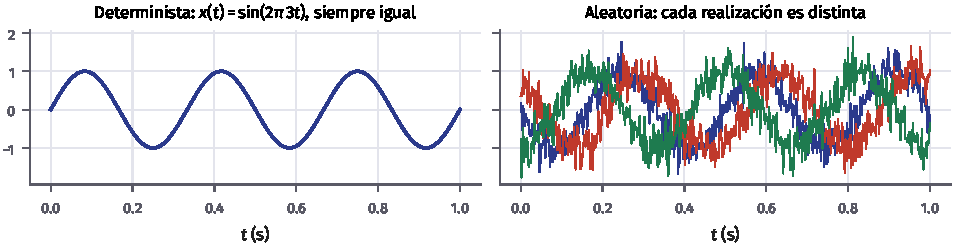
\includegraphics[width=\linewidth]{deterministas_aleatorias}
  \caption{Una señal determinista y tres realizaciones de una señal aleatoria.}\label{fig:det_aleat}
\end{figure}

Una señal aleatoria no se describe valor a valor, sino estadísticamente: qué valores son más probables, cuánto se alejan de su media, cómo se parecen los valores próximos en el tiempo, cómo se reparte su potencia en frecuencia. Para ello se necesita el lenguaje de la probabilidad, que se repasa en esta sección y en la siguiente. Las dos últimas lo aplican a las señales.

\begin{nota}[Erratas de versiones anteriores]
  La introducción antigua tenía varias faltas: «cuantitiva», «guassiana», «area», «Una análisis», «sen» por «seno», y preguntas sin signo de apertura ni tilde («Que», «Como podemos»).
\end{nota}

\subsection{Variable aleatoria}

\begin{definicion}{Variable aleatoria}{va}
  Una \emph{variable aleatoria} $X$ es una función que asigna un número real a cada resultado de un experimento aleatorio. Antes de realizar el experimento solo se sabe con qué probabilidad tomará cada valor; el valor obtenido, $x$, es una \emph{realización} o \emph{muestra} de $X$.
\end{definicion}

Se usan mayúsculas para la variable y minúsculas para sus valores. Una variable es \emph{discreta} si toma valores aislados $x_1,x_2,\dots$ (la cara de un dado, el número de errores en un paquete) y \emph{continua} si toma valores en un intervalo (la tensión de ruido en un instante).

Una variable discreta se describe con su \emph{función de probabilidad}
\[
  p_X(x_i)=P(X=x_i),\qquad p_X(x_i)\ge0,\qquad\sum_ip_X(x_i)=1 .
\]
Para una continua, la probabilidad de un valor concreto es nula, y se usa la \emph{función de densidad} $f_X(x)\ge0$, que da la probabilidad de un intervalo como un área:
\[
  P(a<X\le b)=\int_a^bf_X(x)\dd x,\qquad\int_{-\infty}^{\infty}f_X(x)\dd x=1 .
\]
$f_X(x)\dd x$ es la probabilidad de que $X$ caiga en un intervalo de anchura $\dd x$ alrededor de $x$. La densidad no es una probabilidad y puede valer más que 1: la de $\mathcal U[0;0{,}5]$ vale 2.

Las dos descripciones se unifican con la \emph{función de distribución}
\[
  F_X(x)=P(X\le x),
\]
que es no decreciente, va de $F_X(-\infty)=0$ a $F_X(\infty)=1$ y cumple $P(a<X\le b)=F_X(b)-F_X(a)$. Para una variable continua, $F_X(x)=\int_{-\infty}^xf_X(u)\dd u$ y $f_X=\dd F_X/\dd x$; para una discreta, $F_X$ es una escalera con un salto de altura $p_X(x_i)$ en cada $x_i$ (\cref{fig:pmf}).

\begin{figure}[ht]
  \centering
  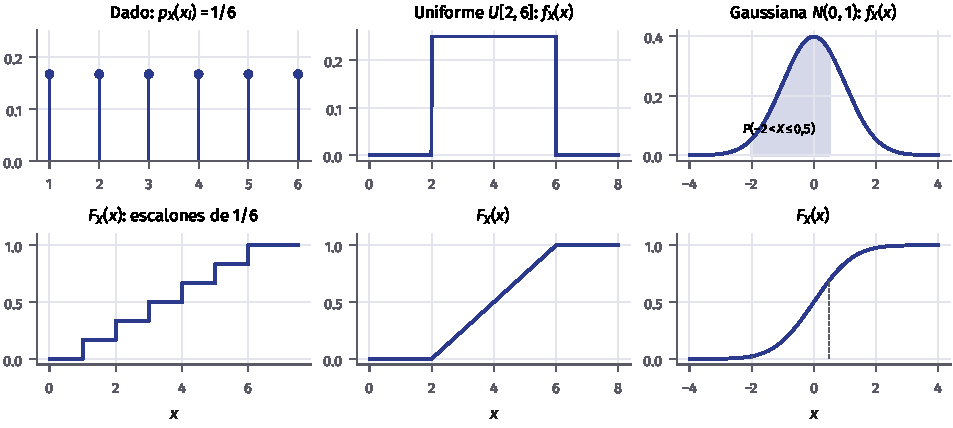
\includegraphics[width=\linewidth]{pmf_pdf_cdf}
  \caption{Función de probabilidad, de densidad y de distribución de un dado, de una uniforme y de una gaussiana.}\label{fig:pmf}
\end{figure}

\subsection{Esperanza, media y varianza}

\begin{definicion}{Esperanza}{esperanza}
  La \emph{esperanza} o valor esperado de $g(X)$ es
  \[
    E\{g(X)\}=\sum_ig(x_i)\,p_X(x_i)\qquad\text{o}\qquad E\{g(X)\}=\int_{-\infty}^{\infty}g(x)\,f_X(x)\dd x .
  \]
\end{definicion}

Es el promedio de $g(X)$ ponderado por la probabilidad. Los casos más usados son:
\begin{itemize}
  \item la \emph{media} $\mu_X=E\{X\}$, el centro de gravedad de la distribución;
  \item el \emph{valor cuadrático medio} $E\{X^2\}$, que, si $X$ es una tensión aplicada a una resistencia de 1\,$\Omega$, es la potencia media;
  \item la \emph{varianza} $\sigma_X^2=E\{(X-\mu_X)^2\}$, que mide la dispersión alrededor de la media. Desarrollando el cuadrado, $\sigma_X^2=E\{X^2\}-\mu_X^2$. Su raíz $\sigma_X$ es la \emph{desviación típica}, con las mismas unidades que $X$.
\end{itemize}
La esperanza es lineal: $E\{aX+b\}=a\mu_X+b$, y de ahí $\operatorname{Var}\{aX+b\}=a^2\sigma_X^2$. Por ejemplo, para un dado equilibrado $\mu_X=3{,}5$, $E\{X^2\}=\frac{1+4+\dots+36}6=\frac{91}6$ y $\sigma_X^2=\frac{91}6-\frac{49}4=\frac{35}{12}$.

\subsection{Distribuciones habituales}

\paragraph{Uniforme.} $X\sim\mathcal U[a,b]$ si su densidad es constante en $[a,b]$:
\[
  f_X(x)=\begin{cases}\dfrac1{b-a},&a\le x\le b,\\0,&\text{en otro caso,}\end{cases}\qquad
  \mu_X=\frac{a+b}2,\quad E\{X^2\}=\frac{a^2+ab+b^2}3,\quad\sigma_X^2=\frac{(b-a)^2}{12}.
\]
Modela el error de cuantificación (Tema~2), la fase de una portadora desconocida y los números aleatorios que genera un ordenador.

\paragraph{Gaussiana o normal.} $X\sim\mathcal N(\mu,\sigma^2)$ si
\[
  f_X(x)=\frac1{\sqrt{2\pi}\,\sigma}\,\e^{-\frac{(x-\mu)^2}{2\sigma^2}} .
\]
Su media es $\mu$ y su varianza $\sigma^2$. La variable $Z=(X-\mu)/\sigma$ es $\mathcal N(0,1)$, cuya función de distribución $\Phi(z)$ está tabulada; así $P(X\le x)=\Phi\big((x-\mu)/\sigma\big)$. A una, dos y tres desviaciones típicas de la media queda el 68,3, el 95,4 y el 99,7\,\% de la probabilidad (\cref{fig:gaussiana}). Una transformación lineal de una gaussiana es gaussiana: $aX+b\sim\mathcal N(a\mu+b,\,a^2\sigma^2)$. Su importancia se debe al teorema del límite central (sección~\ref{sec:tcl}): el ruido que resulta de sumar muchas contribuciones pequeñas e independientes, como el ruido térmico, es gaussiano.

\begin{figure}[ht]
  \centering
  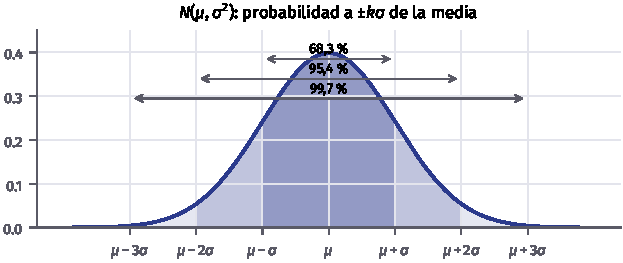
\includegraphics[width=0.66\linewidth]{gaussiana}
  \caption{Densidad gaussiana y probabilidad a $\pm\sigma$, $\pm2\sigma$ y $\pm3\sigma$ de la media.}\label{fig:gaussiana}
\end{figure}

\paragraph{Exponencial.} $f_X(x)=\lambda\e^{-\lambda x}$ para $x\ge0$, con $\mu_X=1/\lambda$ y $\sigma_X^2=1/\lambda^2$. Modela tiempos de espera entre sucesos independientes.

\begin{flushright}\small\color{pdsgris}Ejercicios 1–3.\end{flushright}

\subsection{Muestreo de variables aleatorias}

Los generadores de números pseudoaleatorios de Matlab (\texttt{rand}) y de Python (\texttt{rng.random}, con \texttt{rng = np.random.default\_rng()}) producen muestras de $\mathcal U[0,1)$ que se comportan como independientes. A partir de ellas se pueden obtener muestras de cualquier distribución. Esto permite \emph{simular}: repetir muchas veces un experimento con entradas aleatorias y estimar a partir de los resultados lo que sería difícil de calcular. Es el \emph{método de Monte Carlo}. Fijando la semilla del generador (\texttt{rng(0)} en Matlab, \texttt{default\_rng(0)} en Python) los resultados son reproducibles.

\paragraph{Método de la ruleta.} Para una variable discreta se reparte $[0,1)$ en tramos consecutivos de longitudes $p_X(x_1),p_X(x_2),\dots$, como los sectores de una ruleta, se genera $u\sim\mathcal U[0,1)$ y se devuelve el valor cuyo tramo contiene a $u$:
\[
  x=x_i\qquad\text{si}\qquad F_X(x_{i-1})\le u<F_X(x_i).
\]
Como el tramo $i$ mide $p_X(x_i)$, el valor $x_i$ sale con esa probabilidad.

\begin{encodigo}
  Dado cargado con $p=(0{,}1;\,0{,}1;\,0{,}1;\,0{,}1;\,0{,}1;\,0{,}5)$. Las frecuencias relativas se acercan a $p$ y la media a $4{,}5$.
  \codigo{ruleta}
\end{encodigo}

\paragraph{Inversa de la función de distribución.} Si $U\sim\mathcal U[0,1]$ y $F_X$ es continua y estrictamente creciente, la variable $X=F_X^{-1}(U)$ tiene función de distribución $F_X$, porque
\[
  P(X\le x)=P\big(F_X^{-1}(U)\le x\big)=P\big(U\le F_X(x)\big)=F_X(x).
\]
Para la exponencial, despejando $u=1-\e^{-\lambda x}$ se obtiene $x=-\frac1\lambda\ln(1-u)$ (\cref{fig:inversa}). El método de la ruleta es la versión discreta de este. El resultado también funciona al revés: si $X$ tiene distribución continua $F_X$, la variable $F_X(X)$ es uniforme en $[0,1]$. Es la base de la ecualización del histograma del Tema~5.

\begin{figure}[ht]
  \centering
  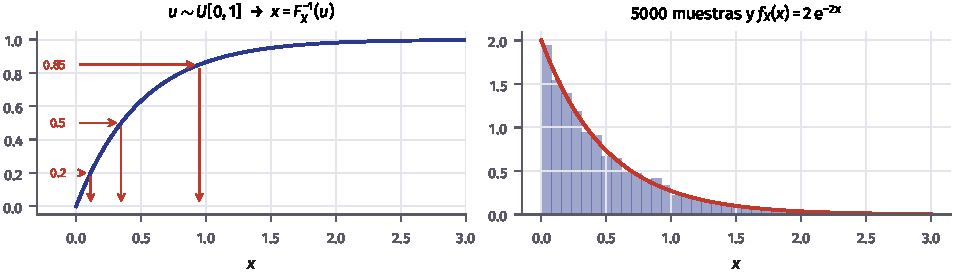
\includegraphics[width=\linewidth]{metodo_inversa}
  \caption{Método de la inversa para la exponencial de $\lambda=2$: tres valores de $u$ y su $x$, y el histograma de 5000 muestras.}\label{fig:inversa}
\end{figure}

\begin{encodigo}
  Muestras exponenciales con $\lambda=2$: la media se acerca a $1/\lambda=0{,}5$, la varianza a $1/\lambda^2=0{,}25$ y la fracción de muestras mayores que 1 a $\e^{-2}=0{,}135$.
  \codigo{muestreo_inversa}
\end{encodigo}

\paragraph{Box-Muller.} La función de distribución de la gaussiana no tiene inversa explícita. Pero un par $(Z_1,Z_2)$ de gaussianas $\mathcal N(0,1)$ independientes, escrito en coordenadas polares, tiene un ángulo $\Theta$ uniforme en $[0,2\pi)$ y un radio $R$ independiente con $F_R(r)=1-\e^{-r^2/2}$ (una distribución de Rayleigh), que sí se puede invertir. Por tanto, con $u_1,u_2\sim\mathcal U[0,1)$ independientes,
\[
  r=\sqrt{-2\ln(1-u_1)},\quad\theta=2\pi u_2,\qquad z_1=r\cos\theta,\quad z_2=r\sin\theta
\]
son dos muestras $\mathcal N(0,1)$ independientes, y $x=\mu+\sigma z$ es $\mathcal N(\mu,\sigma^2)$. En la práctica se usan \texttt{randn} (Matlab) y \texttt{rng.standard\_normal} (Python), que emplean métodos más rápidos.

\begin{encodigo}
  Box-Muller: las dos salidas tienen media 0, desviación típica 1 y están incorreladas; el 68,3\,\% de las muestras cae a menos de una desviación típica.
  \codigo{box_muller}
\end{encodigo}

\paragraph{Aceptación y rechazo.} Cuando $F_X$ no se puede invertir, se busca una densidad $q(x)$ fácil de muestrear y una constante $M$ tales que $Mq(x)\ge f(x)$ para todo $x$. Se genera un candidato $x\sim q$ y un $u\sim\mathcal U[0,1)$, y se \emph{acepta} $x$ si $u\,Mq(x)\le f(x)$; si no, se descarta. Los puntos $(x,\,uMq(x))$ se reparten uniformemente bajo la curva $Mq$, y los aceptados, uniformemente bajo $f$, así que sus abscisas siguen la densidad $f$ (\cref{fig:rechazo}). La fracción aceptada es el cociente de áreas, $1/M$: conviene que $Mq$ se ajuste a $f$.

\begin{figure}[ht]
  \centering
  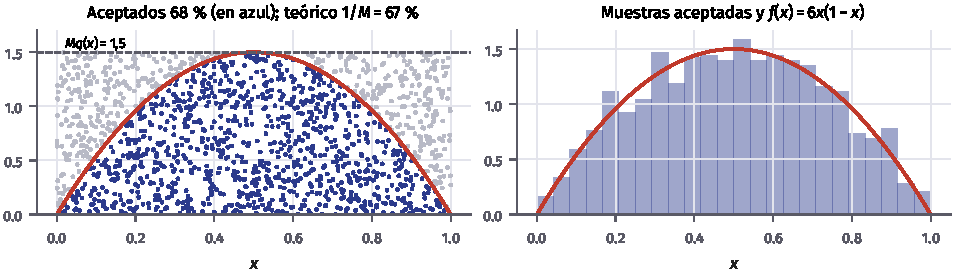
\includegraphics[width=\linewidth]{rechazo}
  \caption{Aceptación y rechazo para $f(x)=6x(1-x)$ en $[0,1]$ con $q$ uniforme y $M=1{,}5$.}\label{fig:rechazo}
\end{figure}

\begin{encodigo}
  Aceptación y rechazo para $f(x)=6x(1-x)$: se acepta un 67\,\% de los candidatos y las muestras tienen media $0{,}5$ y varianza $0{,}05$, las de $f$.
  \codigo{rechazo}
\end{encodigo}

\paragraph{Mezclas.} Una \emph{mezcla} es una combinación convexa de densidades,
\[
  f_X(x)=\sum_{k=1}^K\pi_k\,f_k(x),\qquad\pi_k\ge0,\quad\sum_k\pi_k=1,
\]
que modela poblaciones formadas por varios grupos. Se muestrea en dos pasos: se elige la componente $k$ con probabilidad $\pi_k$ (por el método de la ruleta) y se genera una muestra de $f_k$ (\cref{fig:mezcla}).

\begin{figure}[ht]
  \centering
  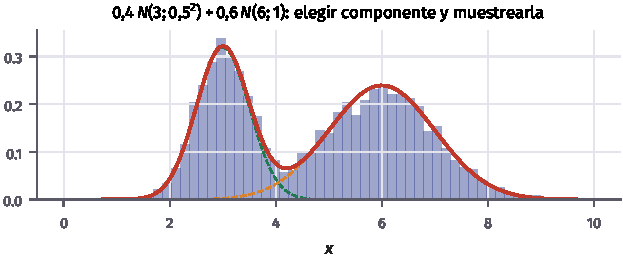
\includegraphics[width=0.66\linewidth]{mezcla}
  \caption{Histograma de 5000 muestras de una mezcla de dos gaussianas.}\label{fig:mezcla}
\end{figure}

\begin{nota}[Erratas de versiones anteriores]
  En la ruleta la condición se escribía con desigualdades estrictas en los dos extremos, de modo que un $u$ igual a un $F_X(x_i)$ no tenía valor asignado. La condición de aceptación y rechazo se escribía $Mq(x)-p(x)>0$; basta $Mq(x)\ge f(x)$. La frase de Box-Muller («Se genera un par…») quedaba sin terminar, y la mezcla del ejemplo, también: «$p_X(x)=0{,}4\mathcal N(x,3,0{,}5)+$».
\end{nota}

\subsection{Análisis de muestras}

\paragraph{Histograma.} Dadas $N$ muestras, se divide el eje en intervalos de anchura $\Delta$ y se cuenta cuántas, $n_j$, caen en cada uno. La altura
\[
  \hat f_X(x)=\frac{n_j}{N\Delta}\qquad\text{para }x\text{ en el intervalo }j
\]
estima la densidad, porque $n_j/N$ estima la probabilidad del intervalo, que es aproximadamente $f_X(x)\Delta$. Con esta normalización el área total es 1 y el histograma se puede comparar con la densidad (\cref{fig:histograma}). Intervalos estrechos dan más detalle pero más ruido, porque cada uno recibe menos muestras. En Matlab, \texttt{histogram(x, 'Normalization', 'pdf')}; en Python, \texttt{plt.hist(x, density=True)}.

\begin{figure}[ht]
  \centering
  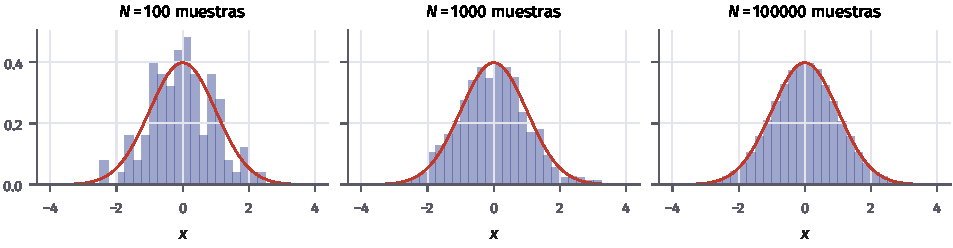
\includegraphics[width=\linewidth]{histograma_n}
  \caption{Histogramas normalizados de muestras $\mathcal N(0,1)$ y la densidad teórica.}\label{fig:histograma}
\end{figure}

\paragraph{Estimadores.} Con $N$ muestras independientes $x_1,\dots,x_N$ de $X$, la media y la varianza se estiman con
\[
  \hat\mu=\frac1N\sum_{i=1}^Nx_i,\qquad\hat\sigma^2=\frac1{N-1}\sum_{i=1}^N(x_i-\hat\mu)^2 .
\]
Un estimador es una variable aleatoria: con otras muestras sale otro valor. $\hat\mu$ es \emph{insesgado}, $E\{\hat\mu\}=\mu$, y su varianza es $\sigma^2/N$; su desviación típica, el error típico de la estimación, decrece como $1/\sqrt N$. Para la varianza se divide por $N-1$ porque las desviaciones se miden respecto a $\hat\mu$, que está más cerca de las muestras que la media verdadera; dividiendo por $N$ el estimador se queda corto en media en un factor $(N-1)/N$. \texttt{var} de Matlab y \texttt{np.var(x, ddof=1)} dividen por $N-1$; \texttt{np.var(x)} y \texttt{var(x, 1)}, por $N$.

\paragraph{Monte Carlo.} De la misma forma, cualquier esperanza se estima con la media de las muestras:
\[
  E\{g(X)\}=\int g(x)\,f_X(x)\dd x\ \approx\ \frac1N\sum_{i=1}^Ng(x_i),
\]
con un error típico de $\sigma_g/\sqrt N$. Así se calculan integrales sin solución cerrada, probabilidades (con $g$ una función indicadora) y el comportamiento de sistemas complejos con entradas aleatorias. La \cref{fig:montecarlo} estima $\pi$ como cuatro veces la fracción de puntos uniformes del cuadrado unidad que caen dentro del cuarto de círculo: para ganar una cifra decimal hace falta cien veces más muestras.

\begin{figure}[ht]
  \centering
  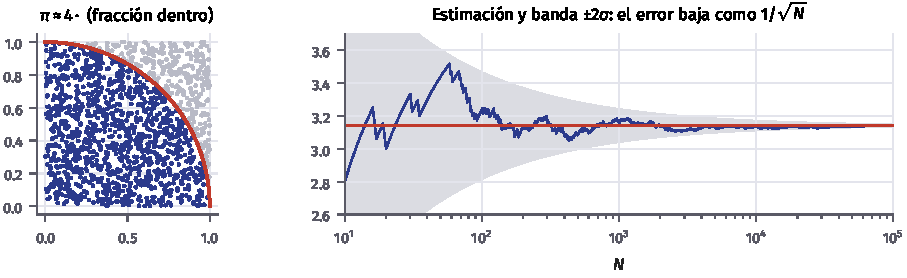
\includegraphics[width=\linewidth]{montecarlo}
  \caption{Estimación de $\pi$ por Monte Carlo y banda de $\pm2$ errores típicos.}\label{fig:montecarlo}
\end{figure}

\begin{encodigo}
  $E\{\cos X\}$ con $X\sim\mathcal N(0,1)$ vale $\e^{-1/2}=0{,}6065$. El error típico estimado baja diez veces al multiplicar $N$ por cien.
  \codigo{montecarlo}
\end{encodigo}

\begin{nota}[Erratas de versiones anteriores]
  La suma de Monte Carlo antigua usaba el índice $n$ y escribía $x_i$ dentro, y el estimador de la varianza dividía por $N$ sin advertir que es sesgado.
\end{nota}

\begin{flushright}\small\color{pdsgris}Ejercicios 4–5.\end{flushright}

% =====================================================================
\section{Varias variables aleatorias}\label{sec:varias}

\subsection{Distribución conjunta}

Muchas magnitudes aleatorias aparecen juntas: el valor de una señal en dos instantes, la entrada y la salida de un sistema, las dos coordenadas de un punto. Para describirlas no basta con cada una por separado; hace falta su \emph{distribución conjunta}:
\[
  F_{XY}(x,y)=P(X\le x,\ Y\le y),\qquad f_{XY}(x,y)=\frac{\partial^2F_{XY}(x,y)}{\partial x\,\partial y},
\]
con $P\big((X,Y)\in A\big)=\iint_Af_{XY}\dd x\dd y$ para cualquier región $A$ del plano. Para variables discretas se usa la probabilidad conjunta $p_{XY}(x_i,y_j)=P(X=x_i,\,Y=y_j)$. Con $M$ variables se escribe $f_{X_1\cdots X_M}(x_1,\dots,x_M)$, o $f_{\mathbf X}(\mathbf x)$ con notación vectorial. Cuando no hay confusión se omiten los subíndices: $f(x,y)$.

\paragraph{Marginales.} La distribución de una sola variable se recupera integrando (o sumando) la conjunta en las demás:
\[
  f_X(x)=\int_{-\infty}^{\infty}f_{XY}(x,y)\dd y,\qquad p_X(x_i)=\sum_jp_{XY}(x_i,y_j).
\]
Con más variables, para obtener la marginal de un subconjunto se integran todas las que no están en él.

\paragraph{Condicionadas.} La densidad de $Y$ sabiendo que $X=x$ es
\[
  f_{Y|X}(y|x)=\frac{f_{XY}(x,y)}{f_X(x)}\qquad(f_X(x)>0).
\]
De aquí salen dos reglas fundamentales:
\begin{itemize}
  \item la \emph{regla de la cadena}, $f_{XY}(x,y)=f_{Y|X}(y|x)\,f_X(x)=f_{X|Y}(x|y)\,f_Y(y)$, que con $M$ variables se escribe
  \[
    f(x_1,\dots,x_M)=f(x_1)\,f(x_2|x_1)\,f(x_3|x_1,x_2)\cdots f(x_M|x_1,\dots,x_{M-1}),
  \]
  y admite $M!$ factorizaciones, una por cada orden de las variables;
  \item el \emph{teorema de Bayes}, que se obtiene igualando las dos factorizaciones:
  \[
    f_{X|Y}(x|y)=\frac{f_{Y|X}(y|x)\,f_X(x)}{f_Y(y)} .
  \]
\end{itemize}

\begin{ejemplo}{Una conjunta construida por partes}{conjunta}
  Sea $X_1\sim\mathcal U[2,4]$ y, dado $X_1=x_1$, $X_2\sim\mathcal N(x_1,1)$. Por la regla de la cadena,
  \[
    f(x_1,x_2)=f(x_2|x_1)\,f(x_1)=\frac12\cdot\frac1{\sqrt{2\pi}}\,\e^{-(x_2-x_1)^2/2},\qquad2\le x_1\le4,
  \]
  y cero fuera (\cref{fig:conjunta}). Para muestrearla se sigue el mismo orden: se genera $x_1$ uniforme y después $x_2=x_1+z$ con $z\sim\mathcal N(0,1)$. Este \emph{muestreo ordenado} según una factorización sirve para cualquier conjunta cuyas condicionadas se sepan muestrear.
\end{ejemplo}

\begin{figure}[ht]
  \centering
  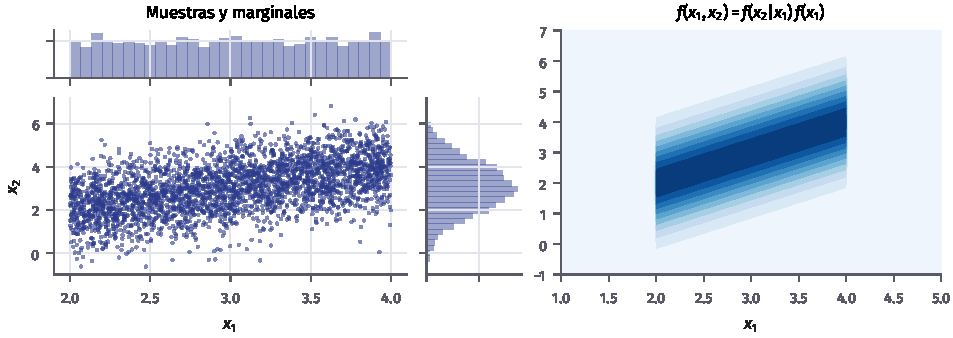
\includegraphics[width=\linewidth]{conjunta}
  \caption{Muestras de la conjunta del ejemplo~\ref{ej:conjunta}, sus histogramas marginales y la densidad conjunta.}\label{fig:conjunta}
\end{figure}

\subsection{Independencia}

\begin{definicion}{Independencia}{independencia}
  $X$ e $Y$ son \emph{independientes} si $f_{XY}(x,y)=f_X(x)\,f_Y(y)$ para todo $(x,y)$, o, equivalentemente, si $f_{Y|X}(y|x)=f_Y(y)$: conocer el valor de $X$ no cambia la distribución de $Y$. $M$ variables son independientes si su conjunta es el producto de las $M$ marginales.
\end{definicion}

Si las variables son independientes, para muestrearlas basta generar cada una por separado. En el ejemplo~\ref{ej:conjunta}, $X_1$ y $X_2$ no son independientes: la media de $X_2$ depende de $X_1$. Se dice que $X$ e $Y$ son \emph{condicionalmente independientes} dado $Z$ si $f_{XY|Z}(x,y|z)=f_{X|Z}(x|z)\,f_{Y|Z}(y|z)$: una vez conocido $Z$, $X$ no aporta nada sobre $Y$. Es la propiedad que define las señales de Markov (sección~\ref{sec:senales}).

\subsection{Correlación y covarianza}

\begin{definicion}{Estadísticos de un par de variables}{estadisticos2}
  \begin{itemize}
    \item \emph{Correlación}: $R_{XY}=E\{XY\}=\displaystyle\iint xy\,f_{XY}(x,y)\dd x\dd y$.
    \item \emph{Covarianza}: $C_{XY}=E\{(X-\mu_X)(Y-\mu_Y)\}=R_{XY}-\mu_X\mu_Y$. Con $Y=X$ es la varianza.
    \item \emph{Coeficiente de correlación}: $\rho_{XY}=\dfrac{C_{XY}}{\sigma_X\,\sigma_Y}$.
  \end{itemize}
\end{definicion}

Por la desigualdad de Cauchy-Schwarz, $-1\le\rho_{XY}\le1$, y $\abs{\rho_{XY}}=1$ si y solo si $Y=aX+b$, con $\rho$ del signo de $a$. El coeficiente mide, por tanto, el grado de dependencia \emph{lineal} (\cref{fig:correlacion}). Se dice que $X$ e $Y$ son \emph{incorreladas} si $C_{XY}=0$, es decir, si $E\{XY\}=\mu_X\mu_Y$, y \emph{ortogonales} si $R_{XY}=0$. La varianza de una suma es
\[
  \operatorname{Var}\{X+Y\}=\sigma_X^2+\sigma_Y^2+2C_{XY},
\]
así que las varianzas se suman cuando las variables están incorreladas.

\begin{figure}[ht]
  \centering
  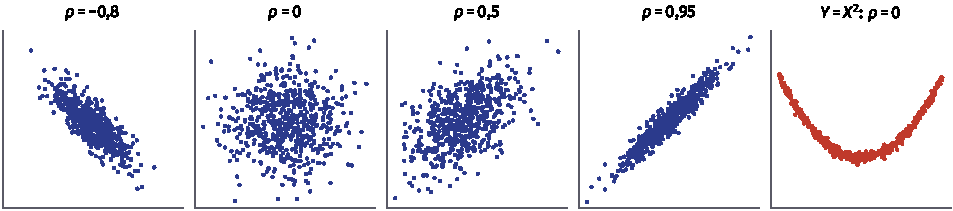
\includegraphics[width=\linewidth]{correlacion}
  \caption{Pares de variables con distintos coeficientes de correlación. En el último, $Y$ depende de $X$ por completo y sin embargo $\rho=0$.}\label{fig:correlacion}
\end{figure}

\begin{propiedad}{Independencia y correlación}{indep-correl}
  Si $X$ e $Y$ son independientes, están incorreladas:
  \[
    E\{XY\}=\iint xy\,f_X(x)f_Y(y)\dd x\dd y=\int xf_X(x)\dd x\int yf_Y(y)\dd y=\mu_X\mu_Y .
  \]
  El recíproco es falso en general.
\end{propiedad}

Con $X\sim\mathcal U[-1,1]$ e $Y=X^2$, $C_{XY}=E\{X^3\}-\mu_X E\{X^2\}=0-0=0$, aunque $Y$ es función de $X$. Por tanto, una correlación distinta de cero prueba que hay dependencia, pero una correlación nula no prueba la independencia. La excepción importante son las variables conjuntamente gaussianas, para las que incorrelación e independencia son equivalentes.

\begin{nota}[Notación y erratas de versiones anteriores]
  Las transparencias antiguas usaban $\phi_{X_iX_j}$ para la correlación y $\psi_{X_iX_j}$ para la covarianza. Aquí se usan $R$ y $C$, porque $\phi$ se reserva para las señales (sección~\ref{sec:senales}) y $\psi$ es la wavelet del Tema~5. Llamaban «independencia lineal» a la incorrelación, que no debe confundirse con la independencia lineal de vectores del álgebra, y escribían $E(X_i,X_j)$ con una coma. La función \texttt{corr} de Matlab que citaban necesita la Statistics Toolbox; \texttt{corrcoef} no.
\end{nota}

\begin{encodigo}
  Estimación de medias, matriz de covarianza y coeficiente de correlación del ejemplo~\ref{ej:conjunta}. Teóricamente $\mu_1=\mu_2=3$, $\sigma_1^2=\frac13$, $\sigma_2^2=1+\frac13$ (la varianza de $X_1$ más la del ruido), $C_{12}=E\{(X_1-3)(X_1-3+Z)\}=\frac13$ y $\rho=\frac{1/3}{\sqrt{1/3\cdot4/3}}=0{,}5$.
  \codigo{conjunta}
\end{encodigo}

\subsection{Vectores aleatorios y gaussiana multivariable}

Con $M$ variables agrupadas en un vector columna $\mathbf X=(X_1,\dots,X_M)^T$, los estadísticos de primer y segundo orden son el \emph{vector de medias} y la \emph{matriz de covarianza}:
\[
  \boldsymbol\mu=E\{\mathbf X\},\qquad
  \boldsymbol\Sigma=E\{(\mathbf X-\boldsymbol\mu)(\mathbf X-\boldsymbol\mu)^T\},\qquad\Sigma_{ij}=C_{X_iX_j},\quad\Sigma_{ii}=\sigma_i^2 .
\]
$\boldsymbol\Sigma$ es simétrica y semidefinida positiva, y diagonal si las variables están incorreladas. Si $\mathbf Y=\mathbf A\mathbf X+\mathbf b$, por la linealidad de la esperanza
\[
  \boldsymbol\mu_Y=\mathbf A\boldsymbol\mu+\mathbf b,\qquad\boldsymbol\Sigma_Y=\mathbf A\boldsymbol\Sigma\mathbf A^T .
\]
Para estimarlos a partir de $N$ muestras se colocan en una matriz de $N\times M$ (una muestra por fila) y se usan \texttt{mean}, \texttt{cov} y \texttt{corrcoef} en Matlab; \texttt{np.cov} y \texttt{np.corrcoef} esperan, por defecto, una variable por fila, de ahí la traspuesta del ejemplo anterior.

\begin{definicion}{Gaussiana multivariable}{gaussiana-mv}
  $\mathbf X\sim\mathcal N(\boldsymbol\mu,\boldsymbol\Sigma)$ si
  \[
    f_{\mathbf X}(\mathbf x)=\frac1{\sqrt{(2\pi)^M\det\boldsymbol\Sigma}}\,\exp\!\Big(-\frac12(\mathbf x-\boldsymbol\mu)^T\boldsymbol\Sigma^{-1}(\mathbf x-\boldsymbol\mu)\Big).
  \]
\end{definicion}

Queda determinada por su media y su covarianza. Sus curvas de nivel son elipses (elipsoides en más dimensiones) centradas en $\boldsymbol\mu$, con los ejes en la dirección de los autovectores de $\boldsymbol\Sigma=\mathbf V\boldsymbol\Lambda\mathbf V^T$ y semiejes proporcionales a $\sqrt{\lambda_k}$ (\cref{fig:gaussiana2d}). Las marginales, las condicionadas y cualquier transformación lineal de una gaussiana son gaussianas. Si $\boldsymbol\Sigma$ es diagonal, la exponencial se factoriza en un producto: incorreladas implica independientes.

\begin{figure}[ht]
  \centering
  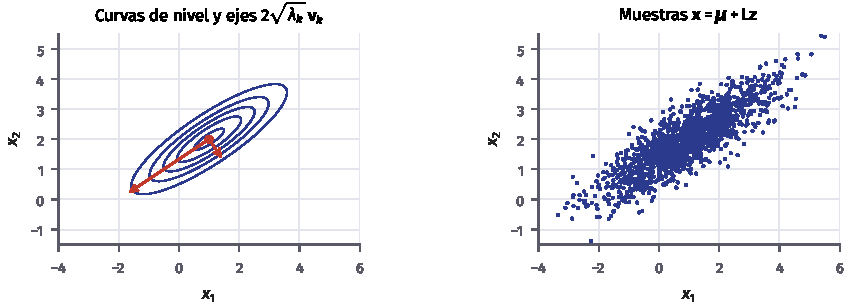
\includegraphics[width=\linewidth]{gaussiana2d}
  \caption{Gaussiana bidimensional con $\boldsymbol\mu=(1,2)^T$ y $\boldsymbol\Sigma=\begin{bsmallmatrix}2&1{,}2\\1{,}2&1\end{bsmallmatrix}$: curvas de nivel con sus ejes, y muestras.}\label{fig:gaussiana2d}
\end{figure}

Para muestrearla se generan $M$ gaussianas independientes $\mathcal N(0,1)$, que forman un vector $\mathbf z$ con covarianza $\mathbf I$, y se transforman:
\[
  \mathbf x=\boldsymbol\mu+\mathbf L\mathbf z,\qquad\mathbf L\mathbf L^T=\boldsymbol\Sigma,
\]
porque entonces $\boldsymbol\Sigma_X=\mathbf L\mathbf I\mathbf L^T=\boldsymbol\Sigma$. $\mathbf L$ puede ser el factor de Cholesky, que se calcula con \texttt{chol(S, 'lower')} en Matlab y con \texttt{np.linalg.cholesky} en Python, o $\mathbf V\boldsymbol\Lambda^{1/2}$, que primero escala cada eje y después gira.

\begin{encodigo}
  Gaussiana bidimensional muestreada con Cholesky. Los autovalores de $\boldsymbol\Sigma$, 0,2 y 2,8, son las varianzas a lo largo de los ejes de la elipse.
  \codigo{gaussiana_nd}
\end{encodigo}

\begin{nota}[Erratas de versiones anteriores]
  La gaussiana multivariable se escribía con $\mathbf x$ como vector fila, $(\mathbf x-\mathbf\mu)\mathbf\Sigma^{-1}(\mathbf x-\mathbf\mu)^T$, y la descomposición de $\mathbf\Sigma$ con \texttt{svd}, sin explicar que para una matriz simétrica definida positiva coincide con la de autovalores. Se decía que la matriz de rotación $\mathbf R$ y la diagonal $\mathbf D$ dan $\mathbf\Sigma=\mathbf R\mathbf D\mathbf R'$, pero no cómo muestrear con ellas: hace falta $\mathbf R\mathbf D^{1/2}$.
\end{nota}

\subsection{Suma de variables y teorema del límite central}\label{sec:tcl}

Sea $S=X+Y$. Por la linealidad, $\mu_S=\mu_X+\mu_Y$ siempre, y $\sigma_S^2=\sigma_X^2+\sigma_Y^2$ si las variables están incorreladas. Si además son independientes, la densidad de la suma es la \emph{convolución} de las densidades:
\[
  f_S(s)=\int_{-\infty}^{\infty}f_X(x)\,f_Y(s-x)\dd x=(f_X\conv f_Y)(s),
\]
porque para que la suma valga $s$ con $X=x$ tiene que ser $Y=s-x$. Por ejemplo, la suma de dos $\mathcal U[0,1]$ independientes tiene densidad triangular en $[0,2]$, la convolución de dos pulsos.

\begin{propiedad}{Teorema del límite central}{tcl}
  Si $X_1,\dots,X_n$ son independientes, con la misma distribución, media $\mu$ y varianza $\sigma^2$ finita, la suma normalizada
  \[
    Z_n=\frac{\sum_{i=1}^nX_i-n\mu}{\sqrt n\,\sigma}
  \]
  tiende a $\mathcal N(0,1)$ cuando $n\to\infty$, cualquiera que sea la distribución de las $X_i$.
\end{propiedad}

La convergencia es rápida (\cref{fig:tcl}): la suma de doce uniformes $\mathcal U[0,1]$ menos 6 tiene media 0 y varianza 1, y ya es casi gaussiana. El teorema se cumple también, con condiciones, para variables no idénticas, y explica por qué el ruido que resulta de sumar muchas contribuciones independientes, como el movimiento de los electrones en una resistencia, es gaussiano.

\begin{figure}[ht]
  \centering
  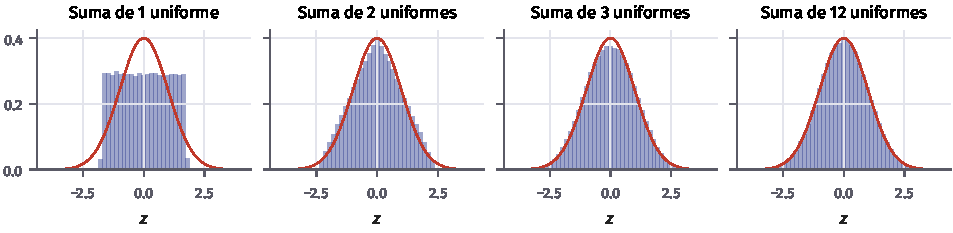
\includegraphics[width=\linewidth]{tcl}
  \caption{Histograma de la suma normalizada de $n$ uniformes y la densidad $\mathcal N(0,1)$.}\label{fig:tcl}
\end{figure}

\begin{flushright}\small\color{pdsgris}Ejercicios 6–10.\end{flushright}

% =====================================================================
\section{Señales aleatorias}\label{sec:senales}

\subsection{Definición y descripción}

\begin{definicion}{Señal aleatoria}{senal-aleatoria}
  Una \emph{señal aleatoria} o \emph{proceso estocástico} es una familia de variables aleatorias indexadas por el tiempo: $x[n]$, $n\in\Z$, en tiempo discreto, o $x(t)$, $t\in\R$, en tiempo continuo.
\end{definicion}

Hay dos formas de verla (\cref{fig:realizaciones}). Fijado el resultado del experimento, se obtiene una señal determinista, una \emph{realización}; fijado el instante $n$, $x[n]$ es una variable aleatoria. El conjunto de todas las realizaciones posibles se llama \emph{conjunto} (\emph{ensemble}). Siguiendo la notación del curso, escribimos la señal aleatoria con minúscula, como sus realizaciones; el contexto aclara de qué se habla.

\begin{figure}[ht]
  \centering
  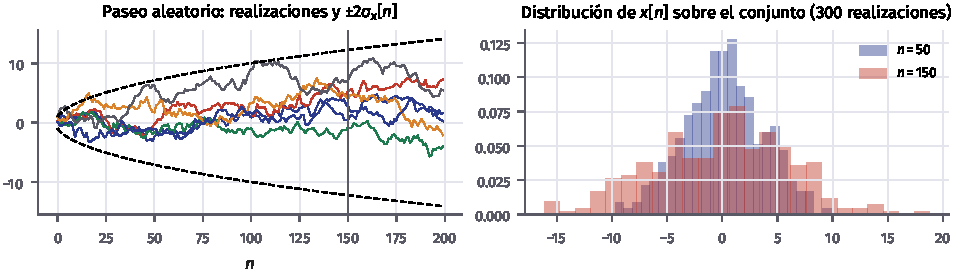
\includegraphics[width=\linewidth]{realizaciones}
  \caption{Seis realizaciones de un paseo aleatorio y la distribución de $x[n]$ en dos instantes, estimada con 300 realizaciones.}\label{fig:realizaciones}
\end{figure}

Una señal aleatoria queda completamente descrita por las distribuciones conjuntas de $x[n_1],\dots,x[n_k]$ para cualesquiera $k$ instantes, algo que casi nunca se conoce. En la práctica se usan los momentos de primer y segundo orden, que son los estadísticos de la sección~\ref{sec:varias} aplicados a los valores de la señal en uno o dos instantes:
\begin{itemize}
  \item media: $\mu_x[n]=E\{x[n]\}$;
  \item valor cuadrático medio o potencia instantánea: $E\{x^2[n]\}$, y varianza $\sigma_x^2[n]=E\{x^2[n]\}-\mu_x^2[n]$;
  \item autocorrelación: $\phi_{xx}[n_1,n_2]=E\{x[n_1]\,x[n_2]\}$;
  \item autocovarianza: $\gamma_{xx}[n_1,n_2]=E\{(x[n_1]-\mu_x[n_1])(x[n_2]-\mu_x[n_2])\}=\phi_{xx}[n_1,n_2]-\mu_x[n_1]\mu_x[n_2]$;
  \item correlación cruzada de dos señales: $\phi_{xy}[n_1,n_2]=E\{x[n_1]\,y[n_2]\}$, y covarianza cruzada $\gamma_{xy}$.
\end{itemize}
En tiempo continuo se definen igual con $x(t_1)$ y $x(t_2)$. Si la señal es \emph{gaussiana}, es decir, si todas sus distribuciones conjuntas son gaussianas, la media y la autocorrelación la describen por completo.

\paragraph{Algunos tipos de señales.}
\begin{itemize}
  \item \emph{I.i.d.}: las $x[n]$ son independientes e idénticamente distribuidas. Si además tienen media nula, son \emph{ruido blanco} (el nombre se explica en la sección~\ref{sec:espectral}): $\phi_{xx}[n_1,n_2]=\sigma^2\delta[n_1-n_2]$.
  \item \emph{De Markov} de primer orden: el futuro solo depende del pasado a través del presente,
  \[
    f(x[n]\,|\,x[n-1],x[n-2],\dots)=f(x[n]\,|\,x[n-1]),
  \]
  de modo que la conjunta se factoriza como $f(x[0],\dots,x[n])=f(x[0])\prod_{k=1}^nf(x[k]\,|\,x[k-1])$, y se muestrea generando cada valor a partir del anterior. Dos ejemplos, con $w[n]$ ruido blanco:
  \begin{itemize}
    \item el \emph{paseo aleatorio} $x[n]=x[n-1]+w[n]$, en el que $f(x[n]|x[n-1])=\mathcal N(x[n-1],\sigma_w^2)$ si $w$ es gaussiano;
    \item la señal \emph{autorregresiva de orden 1}, AR(1): $x[n]=a\,x[n-1]+w[n]$, con $\abs a<1$, que es ruido blanco filtrado por $H(z)=1/(1-az^{-1})$.
  \end{itemize}
  \item En tiempo continuo el papel del retardo lo hace la derivada. El equivalente del AR(1) es la señal que cumple $\dv{x}{t}=-\alpha x(t)+w(t)$ (proceso de Ornstein-Uhlenbeck): ruido blanco a través de un sistema de primer orden.
\end{itemize}

\begin{nota}[Erratas de versiones anteriores]
  La factorización de la señal de Markov omitía el factor $f(x[0])$, y la versión continua se presentaba como «$p(\dot x(t)|x(t))$» sin decir de qué modelo provenía. La primera transparencia decía que la conjunta $p(x(0),\dots,x(10))$ define la señal; hacen falta las conjuntas de cualquier número de instantes.
\end{nota}

\subsection{Estacionariedad}

\begin{definicion}{Señal estacionaria}{estacionaria}
  Una señal es \emph{estacionaria en sentido estricto} si sus distribuciones conjuntas no cambian al desplazar el origen de tiempos. Es \emph{estacionaria en sentido amplio} (ESA) si su media es constante y su autocorrelación solo depende de la separación entre los instantes:
  \[
    \mu_x[n]=\mu_x,\qquad\phi_{xx}[n+l,\,n]=\phi_{xx}[l]\quad\text{para todo }n .
  \]
  Dos señales son \emph{conjuntamente} ESA si cada una lo es y $\phi_{xy}[n+l,n]$ solo depende de $l$.
\end{definicion}

La estacionariedad estricta implica la amplia si los momentos existen; para señales gaussianas las dos son equivalentes. En una señal ESA también son constantes la potencia $E\{x^2[n]\}=\phi_{xx}[0]$ y la varianza. Para señales ESA usaremos, como Oppenheim y Schafer y como la función \texttt{xcorr} de Matlab,
\[
  \phi_{xx}[l]=E\{x[n+l]\,x[n]\},\qquad\phi_{xy}[l]=E\{x[n+l]\,y[n]\},\qquad\gamma_{xx}[l]=\phi_{xx}[l]-\mu_x^2,
\]
y en tiempo continuo $\phi_{xx}(\tau)=E\{x(t+\tau)\,x(t)\}$.

\begin{ejemplo}{¿Cuáles son estacionarias?}{estacionarias}
  (\Cref{fig:estacionariedad}.)
  \begin{enumerate}
    \item i.i.d.\ $\mathcal U[0,1]$: estacionaria. $\mu_x=\frac12$, $\phi_{xx}[0]=E\{x^2\}=\frac13$ y $\phi_{xx}[l]=\mu_x^2=\frac14$ para $l\ne0$, porque valores distintos son independientes.
    \item Independientes $\mathcal N(0,\sigma^2[n])$ con $\sigma[n]=0{,}97^n$: no estacionaria, porque la varianza depende de $n$, aunque los valores sean independientes.
    \item Paseo aleatorio con $x[0]=0$: $x[n]=\sum_{k=1}^nw[k]$, así que $\mu_x=0$ pero $\operatorname{Var}\{x[n]\}=n\sigma_w^2$ crece con $n$: no estacionaria.
    \item Constante aleatoria $x[n]=A$ con $A\sim\mathcal U[0,1]$: estacionaria, con $\mu_x=\frac12$ y $\phi_{xx}[l]=E\{A^2\}=\frac13$ para todo $l$.
  \end{enumerate}
\end{ejemplo}

\begin{figure}[ht]
  \centering
  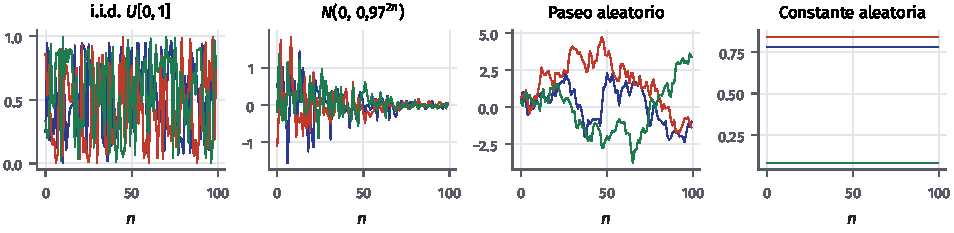
\includegraphics[width=\linewidth]{estacionariedad}
  \caption{Tres realizaciones de las cuatro señales del ejemplo~\ref{ej:estacionarias}.}\label{fig:estacionariedad}
\end{figure}

\begin{ejemplo}{Sinusoide de fase aleatoria}{fase}
  Sea $x[n]=A\cos(\Omega_0n+\theta)$ con $A$ y $\Omega_0$ fijos y $\theta\sim\mathcal U[0,2\pi)$. Su media es $\frac{A}{2\pi}\int_0^{2\pi}\cos(\Omega_0n+\theta)\dd\theta=0$, y, usando $\cos\alpha\cos\beta=\frac12[\cos(\alpha+\beta)+\cos(\alpha-\beta)]$,
  \[
    \phi_{xx}[n+l,n]=\frac{A^2}2E\{\cos(\Omega_0(2n+l)+2\theta)\}+\frac{A^2}2\cos(\Omega_0l)=\frac{A^2}2\cos(\Omega_0l),
  \]
  porque el primer término promedia un coseno sobre una fase uniforme. Es ESA, y su autocorrelación es periódica y no se amortigua (\cref{fig:fase}).
\end{ejemplo}

\begin{figure}[ht]
  \centering
  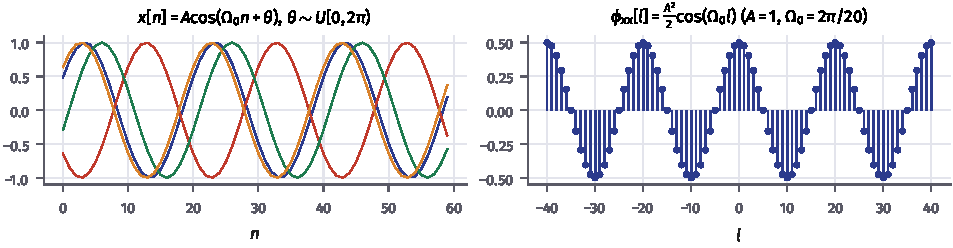
\includegraphics[width=\linewidth]{fase_aleatoria}
  \caption{Realizaciones de una sinusoide de fase aleatoria y su autocorrelación.}\label{fig:fase}
\end{figure}

\begin{nota}[Erratas de versiones anteriores]
  La definición antigua de estacionariedad en sentido amplio era «la función de probabilidad no depende del tiempo: $p(x(t_1))=p(x(t_2))$». Eso es una condición sobre la distribución de primer orden completa, que no basta para la ESA (no dice nada de la autocorrelación) ni es necesaria (una señal ESA puede cambiar de distribución si conserva media y varianza). Los ejemplos hablaban de «sistema discreto» donde querían decir señal.
\end{nota}

\subsection{Ergodicidad}

En la práctica casi nunca se dispone de muchas realizaciones, sino de una sola grabación. La pregunta es si los estadísticos, que son promedios sobre el conjunto, se pueden obtener promediando en el tiempo una única realización.

\begin{definicion}{Ergodicidad}{ergodica}
  Una señal ESA es \emph{ergódica} (en media y en autocorrelación) si, para casi todas sus realizaciones,
  \[
    \lim_{N\to\infty}\frac1{2N+1}\sum_{n=-N}^Nx[n]=\mu_x,\qquad
    \lim_{N\to\infty}\frac1{2N+1}\sum_{n=-N}^Nx[n+l]\,x[n]=\phi_{xx}[l].
  \]
  En tiempo continuo, igual con $\frac1{2T}\int_{-T}^{T}$ y $T\to\infty$.
\end{definicion}

Intuitivamente, una realización larga recorre todos los comportamientos posibles de la señal. Las señales i.i.d., las AR(1) estacionarias y la sinusoide de fase aleatoria son ergódicas. La constante aleatoria del ejemplo~\ref{ej:estacionarias} es estacionaria pero no ergódica: el promedio temporal de una realización es el valor $A$ que le tocó, no $\frac12$. Una condición suficiente para la ergodicidad en media es que $\gamma_{xx}[l]\to0$ cuando $\abs l\to\infty$. Salvo que se diga lo contrario, supondremos que las señales estacionarias son ergódicas, y estimaremos sus estadísticos a partir de una realización.

\subsection{Autocorrelación}

\begin{propiedad}{Propiedades de la autocorrelación de una señal ESA real}{prop-autocorr}
  \begin{itemize}
    \item $\phi_{xx}[0]=E\{x^2[n]\}=\sigma_x^2+\mu_x^2$ es la potencia media de la señal.
    \item Es par: $\phi_{xx}[-l]=E\{x[n-l]\,x[n]\}=\phi_{xx}[l]$ (basta cambiar $n$ por $n+l$).
    \item Tiene el máximo en el origen: $\abs{\phi_{xx}[l]}\le\phi_{xx}[0]$, por Cauchy-Schwarz.
    \item Si la señal no tiene componentes periódicas ni constantes aleatorias, los valores muy separados son incorrelados: $\gamma_{xx}[l]\to0$ y $\phi_{xx}[l]\to\mu_x^2$ cuando $\abs l\to\infty$.
  \end{itemize}
\end{propiedad}

La última propiedad sirve para detectar componentes deterministas: si la autocorrelación no tiende a $\mu_x^2$, la señal tiene una parte determinista, y si esta es periódica, $\phi_{xx}$ oscila con el mismo periodo. La \cref{fig:autocorr} muestra cuatro casos con $T_s=0{,}01$\,s y 10\,s de señal: ruido i.i.d.\ $\mathcal N(5,1)$, con un pico de $\sigma^2+\mu^2=26$ en el origen y $\mu^2=25$ fuera; ruido i.i.d.\ $\mathcal U[2,6]$, con $E\{x^2\}=\frac{4+12+36}3=17{,}3$ y $\mu^2=16$; un seno, cuya autocorrelación oscila sin amortiguarse, y un AR(1) con $a=0{,}95$, cuya autocorrelación decae exponencialmente.

\begin{figure}[ht]
  \centering
  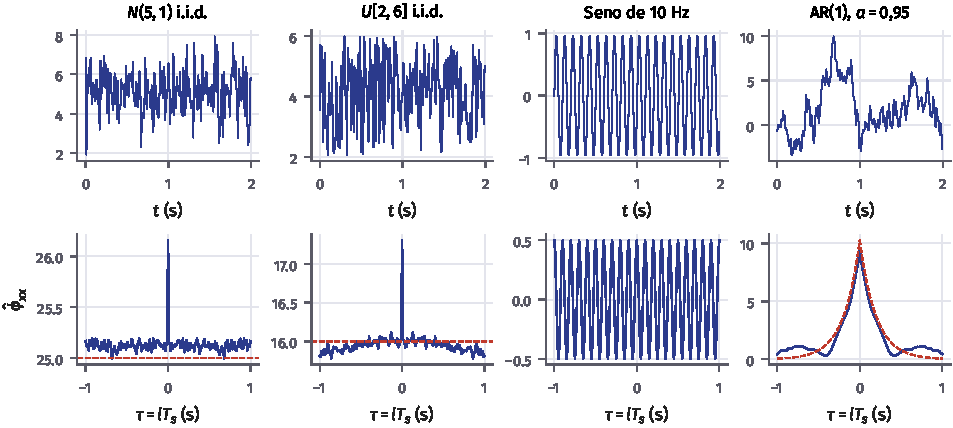
\includegraphics[width=\linewidth]{autocorrelacion_ejemplos}
  \caption{Cuatro señales y su autocorrelación estimada. En rojo, los valores teóricos.}\label{fig:autocorr}
\end{figure}

\begin{nota}[Erratas de versiones anteriores]
  Se escribía «$\phi_{XX}(0)>\phi_{XX}(\tau)$»; la desigualdad correcta es $\phi_{xx}(0)\ge\abs{\phi_{xx}(\tau)}$, con igualdad posible (una sinusoide la alcanza en cada periodo). El límite $\phi_{xx}\to\mu_x^2$ se daba «para $t\gg0$» en lugar de para $\abs\tau\to\infty$, se presentaba como una propiedad de toda señal estacionaria, y la nota de la deducción de la salida de un sistema LTI llamaba $\psi_{XX}$ a la autocorrelación.
\end{nota}

\paragraph{Estimación.} Con una realización de $N$ muestras $x[0],\dots,x[N-1]$ de una señal ergódica, hay $N-\abs l$ productos $x[n+\abs l]\,x[n]$ disponibles para la separación $l$. Su media es el estimador \emph{insesgado}
\[
  \hat\phi_{xx}[l]=\frac1{N-\abs l}\sum_{n=0}^{N-1-\abs l}x[n+\abs l]\,x[n],
\]
y si se divide por $N$ se obtiene el estimador \emph{sesgado} $\check\phi_{xx}[l]=\frac{N-\abs l}N\hat\phi_{xx}[l]$. El insesgado acierta en media, pero para $\abs l$ cercano a $N$ promedia muy pocos productos y es muy ruidoso; el sesgado se amortigua hacia los extremos y tiene menos varianza, y su transformada de Fourier es siempre no negativa (sección~\ref{sec:espectral}). En cualquier caso, solo tiene sentido para $\abs l$ bastante menor que $N$. En Matlab, \texttt{xcorr(x, L, 'unbiased')} o \texttt{'biased'} calculan los valores para $\abs l\le L$; en Python se usa \texttt{np.correlate(x, x, 'full')} y se divide por el número de productos.

\begin{encodigo}
  Autocorrelación estimada de ruido i.i.d.\ $\mathcal N(5,1)$ y $\mathcal U[2,6]$ con 1001 muestras: en el origen, unos 26 y 17,3; a 50 muestras, unos 25 y 16.
  \codigo{autocorrelacion}
\end{encodigo}

\begin{ejemplo}{Autocorrelación de un AR(1)}{ar1}
  Sea $x[n]=a\,x[n-1]+w[n]$, con $\abs a<1$ y $w$ ruido blanco de varianza $\sigma_w^2$, en régimen estacionario. Como $x[n-1]$ solo depende de $w[n-1],w[n-2],\dots$, es independiente de $w[n]$, y
  \[
    \sigma_x^2=E\{(ax[n-1]+w[n])^2\}=a^2\sigma_x^2+\sigma_w^2\ \Rightarrow\ \sigma_x^2=\frac{\sigma_w^2}{1-a^2}.
  \]
  Para $l>0$, $\phi_{xx}[l]=E\{(ax[n+l-1]+w[n+l])\,x[n]\}=a\,\phi_{xx}[l-1]$, y por ser par,
  \[
    \phi_{xx}[l]=\frac{\sigma_w^2}{1-a^2}\,a^{\abs l}.
  \]
  Con $a$ cerca de 1 los valores están muy correlados y la señal varía despacio; con $a<0$ la autocorrelación alterna de signo y la señal cambia de signo con frecuencia.
\end{ejemplo}

\begin{encodigo}
  Autocorrelación de un AR(1) con $a=0{,}9$ comparada con la teórica. La potencia, $1/(1-0{,}81)=5{,}26$, es cinco veces la del ruido de entrada.
  \codigo{ar1}
\end{encodigo}

\subsection{Correlación cruzada}

$\phi_{xy}[l]=E\{x[n+l]\,y[n]\}$ mide cuánto se parece $x$, adelantada $l$ muestras, a $y$. A diferencia de la autocorrelación, no tiene por qué ser par ni tener el máximo en el origen.

\begin{propiedad}{Propiedades de la correlación cruzada}{prop-cruzada}
  Para dos señales reales conjuntamente ESA:
  \begin{itemize}
    \item $\phi_{xy}[l]=\phi_{yx}[-l]$;
    \item $\abs{\phi_{xy}[l]}^2\le\phi_{xx}[0]\,\phi_{yy}[0]$ y $\abs{\phi_{xy}[l]}\le\frac12\big(\phi_{xx}[0]+\phi_{yy}[0]\big)$;
    \item si $x$ e $y$ son independientes (o incorreladas), $\phi_{xy}[l]=\mu_x\mu_y$ para todo $l$.
  \end{itemize}
\end{propiedad}

\begin{ejemplo}{Eco}{eco}
  Una señal $x$ blanca de varianza $\sigma_x^2$ se recibe con un retardo $D$, atenuada y con ruido $v$ independiente: $y[n]=\alpha\,x[n-D]+v[n]$. Entonces
  \[
    \phi_{yx}[l]=E\{y[n+l]\,x[n]\}=\alpha\,E\{x[n+l-D]\,x[n]\}+E\{v[n+l]\}E\{x[n]\}=\alpha\sigma_x^2\,\delta[l-D]:
  \]
  la correlación cruzada tiene un pico en el retardo. Si $x$ no es blanca, el pico tiene la forma de $\phi_{xx}$ centrada en $D$.
\end{ejemplo}

Esta es la base de muchas aplicaciones: medir distancias con radar o sonar (se correla el eco con el pulso emitido), localizar una fuente con dos micrófonos, detectar los caminos de propagación de un canal (un pico por camino) o sincronizar un receptor con una trama conocida. En la \cref{fig:retardo} se busca $x(t)=\sinc(t-2)$ dentro de $y(t)=\sinc(t-3)$ más ruido gaussiano de desviación típica 1; aunque el pulso apenas se distingue, la correlación cruzada tiene el máximo en $\tau\approx1$\,s.

\begin{figure}[ht]
  \centering
  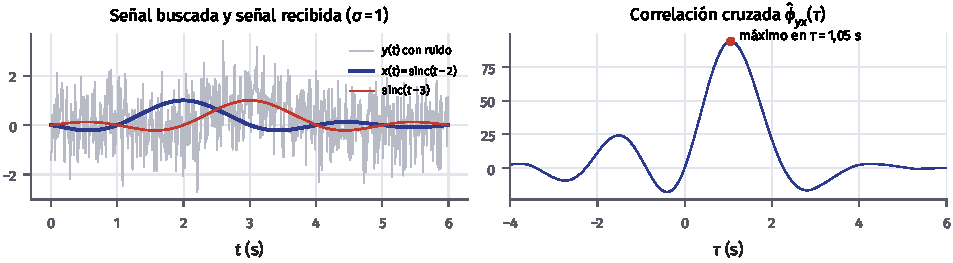
\includegraphics[width=\linewidth]{retardo}
  \caption{Estimación de un retardo con la correlación cruzada.}\label{fig:retardo}
\end{figure}

\begin{encodigo}
  Estimación del retardo. \texttt{xcorr(y, x)} y \texttt{np.correlate(y, x, 'full')} calculan $\sum_ny[n+l]\,x[n]$, es decir, $\phi_{yx}$ salvo el factor de normalización.
  \codigo{retardo}
\end{encodigo}

\begin{nota}[Convenio de la correlación cruzada]
  Las transparencias antiguas, y otros textos, definen $\phi_{xy}(\tau)=E\{x(t)\,y(t+\tau)\}$, que es la función de estos apuntes reflejada, $\phi_{xy}(-\tau)$, o lo que es lo mismo, $\phi_{yx}(\tau)$. Con aquel convenio la relación de un sistema LTI se escribe $\Phi_{xy}=H\Phi_{xx}$; con este, $\Phi_{yx}=H\Phi_{xx}$. Seguimos el de Oppenheim y Schafer y Matlab.
\end{nota}

\begin{flushright}\small\color{pdsgris}Ejercicios 11–14.\end{flushright}

% =====================================================================
\section{Análisis espectral de señales aleatorias}\label{sec:espectral}

\subsection{Densidad espectral de potencia}

Una realización de una señal estacionaria no decae: tiene energía infinita, y su DTFT no existe en sentido ordinario. Además, cada realización tendría una transformada distinta. Lo que sí está bien definido es la potencia media,
\[
  P_x=E\Big\{\lim_{N\to\infty}\frac1{2N+1}\sum_{n=-N}^Nx^2[n]\Big\}=\lim_{N\to\infty}\frac1{2N+1}\sum_{n=-N}^NE\{x^2[n]\}=\phi_{xx}[0]\quad\text{(señal ESA)},
\]
y, más en general, la autocorrelación, que es como una potencia que depende de la separación $l$. Su transformada de Fourier describe cómo se reparte la potencia en frecuencia.

\begin{definicion}{Densidad espectral de potencia}{dep}
  La \emph{densidad espectral de potencia} (DEP), o espectro de potencia, de una señal ESA es la DTFT de su autocorrelación:
  \[
    \Phi_{xx}(\e^{j\Omega})=\sum_{l=-\infty}^{\infty}\phi_{xx}[l]\,\e^{-j\Omega l},\qquad
    \phi_{xx}[l]=\frac1{2\pi}\int_{-\pi}^{\pi}\Phi_{xx}(\e^{j\Omega})\,\e^{j\Omega l}\dd\Omega .
  \]
  En tiempo continuo, $\Phi_{xx}(j\omega)=\int_{-\infty}^{\infty}\phi_{xx}(\tau)\,\e^{-j\omega\tau}\dd\tau$.
\end{definicion}

\begin{propiedad}{Propiedades de la DEP}{prop-dep}
  \begin{itemize}
    \item La potencia es el área: $P_x=\phi_{xx}[0]=\dfrac1{2\pi}\displaystyle\int_{-\pi}^{\pi}\Phi_{xx}(\e^{j\Omega})\dd\Omega$.
    \item Es real, porque $\phi_{xx}$ es par; par en $\Omega$ si $x$ es real; y no negativa.
    \item Teorema de Wiener-Khinchin: si $X_N(\e^{j\Omega})$ es la DTFT de $2N+1$ muestras de una realización,
    \[
      \Phi_{xx}(\e^{j\Omega})=\lim_{N\to\infty}\frac1{2N+1}E\big\{\abs{X_N(\e^{j\Omega})}^2\big\}.
    \]
  \end{itemize}
\end{propiedad}

El tercer punto justifica el nombre: $\Phi_{xx}$ es el cuadrado del módulo del espectro, por unidad de tiempo y promediado sobre las realizaciones. La potencia contenida en la banda $\Omega_1\le\abs\Omega\le\Omega_2$ es $\frac1{2\pi}$ por la integral de $\Phi_{xx}$ en esa banda, contando las frecuencias positivas y negativas. En tiempo continuo, $P_x=\frac1{2\pi}\int\Phi_{xx}(j\omega)\dd\omega=\int\Phi_{xx}(j2\pi f)\dd f$, de modo que $\Phi_{xx}$ se mide en W/Hz si $x$ es una tensión sobre 1\,$\Omega$.

\begin{ejemplo}{Densidades espectrales}{deps}
  \begin{itemize}
    \item \emph{Ruido blanco} de varianza $\sigma^2$: $\phi_{xx}[l]=\sigma^2\delta[l]$ y $\Phi_{xx}(\e^{j\Omega})=\sigma^2$. Todas las frecuencias tienen la misma potencia, como la luz blanca contiene todos los colores; de ahí el nombre.
    \item \emph{AR(1)}: de $\phi_{xx}[l]=\frac{\sigma_w^2}{1-a^2}a^{\abs l}$,
    \[
      \Phi_{xx}(\e^{j\Omega})=\frac{\sigma_w^2}{1-a^2}\left(\frac1{1-a\e^{-j\Omega}}+\frac1{1-a\e^{j\Omega}}-1\right)=\frac{\sigma_w^2}{\abs{1-a\e^{-j\Omega}}^2}=\frac{\sigma_w^2}{1-2a\cos\Omega+a^2}.
    \]
    Paso bajo si $a>0$ y paso alto si $a<0$ (\cref{fig:dep}).
    \item \emph{Constante} $\mu$ (o componente continua): $\phi_{xx}[l]=\mu^2$ y $\Phi_{xx}=2\pi\mu^2\delta(\Omega)$ en $[-\pi,\pi]$, repetida con periodo $2\pi$.
    \item \emph{Sinusoide de fase aleatoria}: $\phi_{xx}[l]=\frac{A^2}2\cos\Omega_0l$ y $\Phi_{xx}=\frac{\pi A^2}2\big[\delta(\Omega-\Omega_0)+\delta(\Omega+\Omega_0)\big]$: toda la potencia, $A^2/2$, en $\pm\Omega_0$.
  \end{itemize}
\end{ejemplo}

\begin{figure}[ht]
  \centering
  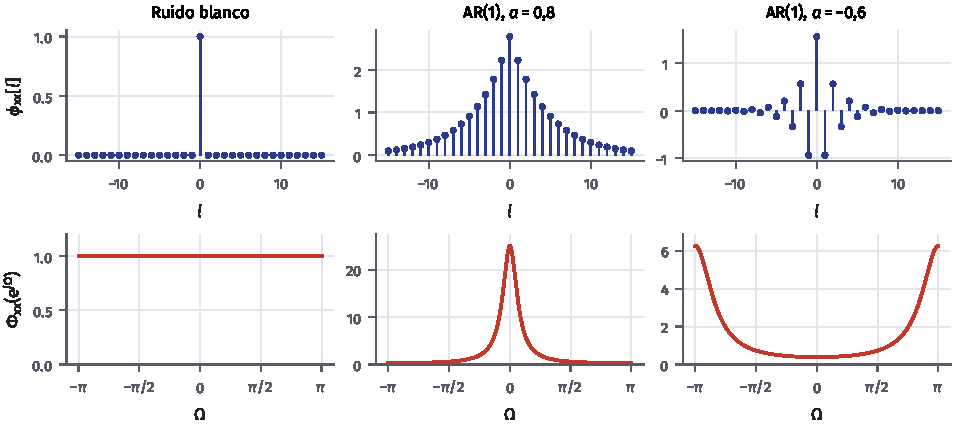
\includegraphics[width=\linewidth]{dep_ejemplos}
  \caption{Autocorrelación y densidad espectral de potencia de ruido blanco y de dos AR(1), con $\sigma_w^2=1$.}\label{fig:dep}
\end{figure}

Según la forma de su DEP, las señales se clasifican en \emph{blancas} (DEP plana), \emph{coloreadas} (cualquier otra), de \emph{banda ancha} o de \emph{banda estrecha}, \emph{paso bajo} o \emph{paso banda}. Como en cualquier par transformado, la anchura de la autocorrelación es inversa al ancho de banda: una señal de banda estrecha tiene valores correlados a gran distancia.

\begin{importante}[Ruido blanco en tiempo continuo]
  El ruido blanco continuo tiene $\phi_{xx}(\tau)=\frac{N_0}2\delta(\tau)$ y $\Phi_{xx}(j\omega)=\frac{N_0}2$. Su potencia, $\phi_{xx}(0)$, es infinita, así que no existe físicamente: es un modelo de un ruido cuya DEP es plana en toda la banda que interesa. El ruido térmico de una resistencia $R$ a temperatura $T$ tiene $N_0/2=2kTR$\,V$^2$/Hz hasta frecuencias de teraherzios. Tras un paso bajo ideal de $B$\,Hz la potencia es $\frac{N_0}2\cdot2B=N_0B$, y si esa señal se muestrea a $f_s=2B$ resulta ruido blanco discreto de varianza $N_0B$.
\end{importante}

\begin{nota}[Erratas de versiones anteriores]
  Las transparencias antiguas usaban $\omega$ para la frecuencia discreta, escribían la DEP de una constante como $\mu^2\delta(\omega)$, sin el factor $2\pi$, y llamaban «bias constante» a la componente continua.
\end{nota}

\paragraph{Densidad espectral cruzada.} Es la DTFT de la correlación cruzada:
\[
  \Phi_{xy}(\e^{j\Omega})=\sum_{l=-\infty}^{\infty}\phi_{xy}[l]\,\e^{-j\Omega l}.
\]
En general es compleja, porque $\phi_{xy}$ no es par; como $\phi_{yx}[l]=\phi_{xy}[-l]$, para señales reales $\Phi_{yx}=\Phi_{xy}^*$. Su módulo indica en qué frecuencias tienen $x$ e $y$ potencia en común, y su fase, el desfase entre ellas. La \emph{coherencia}
\[
  C_{xy}(\e^{j\Omega})=\frac{\abs{\Phi_{xy}(\e^{j\Omega})}^2}{\Phi_{xx}(\e^{j\Omega})\,\Phi_{yy}(\e^{j\Omega})}\in[0,1]
\]
vale 1 en las frecuencias en las que $y$ es una versión filtrada de $x$ sin ruido y 0 donde no tienen nada en común.

\subsection{Respuesta de un sistema LTI}

Sea $y[n]=\sum_kh[k]\,x[n-k]$ la salida de un sistema LTI estable, con $h$ real y determinista, a una entrada $x$ ESA. Toda la aleatoriedad está en la señal. Por la linealidad de la esperanza:

\begin{itemize}
  \item \emph{Media}:
  \[
    \mu_y=E\Big\{\sum_kh[k]\,x[n-k]\Big\}=\sum_kh[k]\,E\{x[n-k]\}=\mu_x\sum_kh[k]=H(\e^{j0})\,\mu_x .
  \]
  \item \emph{Correlación cruzada salida-entrada}:
  \[
    \phi_{yx}[l]=E\{y[n+l]\,x[n]\}=\sum_kh[k]\,E\{x[n+l-k]\,x[n]\}=\sum_kh[k]\,\phi_{xx}[l-k]=(h\conv\phi_{xx})[l].
  \]
  \item \emph{Autocorrelación de la salida}:
  \[
    \phi_{yy}[l]=E\Big\{\sum_kh[k]x[n+l-k]\sum_rh[r]x[n-r]\Big\}=\sum_k\sum_rh[k]\,h[r]\,\phi_{xx}[l-k+r].
  \]
  Con $c[m]=\sum_rh[r]\,h[r+m]=(h\conv\tilde h)[m]$, $\tilde h[n]=h[-n]$, y el cambio $m=k-r$, queda $\phi_{yy}[l]=\sum_mc[m]\,\phi_{xx}[l-m]=(h\conv\tilde h\conv\phi_{xx})[l]$.
\end{itemize}

Ninguno depende de $n$: la salida es ESA, y conjuntamente ESA con la entrada. En frecuencia las convoluciones se convierten en productos, y como la DTFT de $\tilde h$ es $H(\e^{-j\Omega})=H^*(\e^{j\Omega})$:

\begin{propiedad}{Señal aleatoria a través de un sistema LTI}{lti}
  \[
    \mu_y=H(\e^{j0})\,\mu_x,\qquad
    \Phi_{yx}(\e^{j\Omega})=H(\e^{j\Omega})\,\Phi_{xx}(\e^{j\Omega}),\qquad
    \Phi_{yy}(\e^{j\Omega})=\abs{H(\e^{j\Omega})}^2\,\Phi_{xx}(\e^{j\Omega}).
  \]
  La potencia de salida es $P_y=\frac1{2\pi}\int_{-\pi}^{\pi}\abs{H(\e^{j\Omega})}^2\,\Phi_{xx}(\e^{j\Omega})\dd\Omega$; con entrada blanca de varianza $\sigma_x^2$, $P_y=\sigma_x^2\sum_kh^2[k]$.
\end{propiedad}

En tiempo continuo se cumple lo mismo con $H(j\omega)$. Un filtro no crea potencia en frecuencias donde no la había: solo multiplica la de cada frecuencia por $\abs H^2$. Al revés, filtrando ruido blanco con el $H$ adecuado se obtiene ruido con la DEP que se quiera, $\Phi_{yy}=\sigma_x^2\abs H^2$ (\cref{fig:filtrado}): es como se simulan perturbaciones realistas, y el AR(1) no es más que ruido blanco tras $1/(1-az^{-1})$. Un filtro \emph{blanqueador} $1/H$, si es estable, convierte ese ruido coloreado otra vez en blanco.

\begin{figure}[ht]
  \centering
  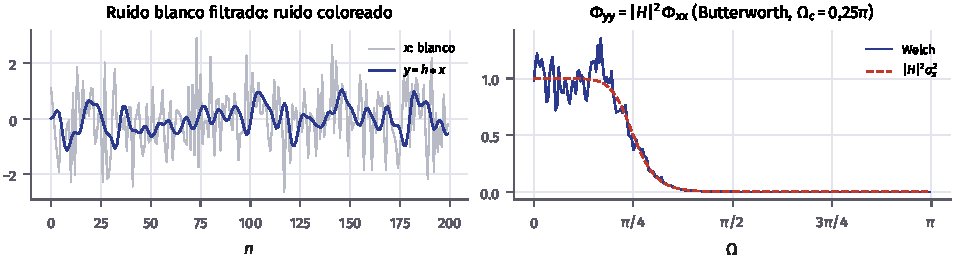
\includegraphics[width=\linewidth]{filtrado_ruido}
  \caption{Ruido blanco a través de un Butterworth discreto de orden 4: realización y DEP de la salida estimada con el método de Welch.}\label{fig:filtrado}
\end{figure}

\begin{nota}[Erratas de versiones anteriores]
  La relación se escribía $\Phi_{YY}=\abs{H(\e^{j\omega})H(\e^{-j\omega})}\Phi_{XX}$: el resultado es correcto para $h$ real, pero el valor absoluto sobra y oculta que $H(\e^{-j\Omega})=H^*(\e^{j\Omega})$. La deducción usaba $\psi_{XX}$ para la autocorrelación, y la diapositiva decía «Ss pueden procesar» y «aleatoreidad».
\end{nota}

\paragraph{Identificación de sistemas.} Las relaciones anteriores permiten medir la respuesta en frecuencia de un sistema desconocido: se le aplica una entrada aleatoria y se miden entrada y salida. De $\Phi_{yx}=H\Phi_{xx}$,
\[
  \hat H(\e^{j\Omega})=\frac{\Phi_{yx}(\e^{j\Omega})}{\Phi_{xx}(\e^{j\Omega})},
\]
que da el módulo y la fase. Si la salida se mide con un ruido $v$ incorrelado con la entrada, $\Phi_{yx}$ no cambia, porque $\phi_{vx}=0$; en cambio $\Phi_{yy}$ aumenta en $\Phi_{vv}$, así que $\abs H^2=\Phi_{yy}/\Phi_{xx}$ daría un resultado sesgado, y además sin fase. Con entrada blanca, $\phi_{yx}[l]=\sigma_x^2h[l]$: la correlación cruzada es la respuesta al impulso. La \cref{fig:identificacion} muestra el resultado para un sistema de segundo orden.

\begin{figure}[ht]
  \centering
  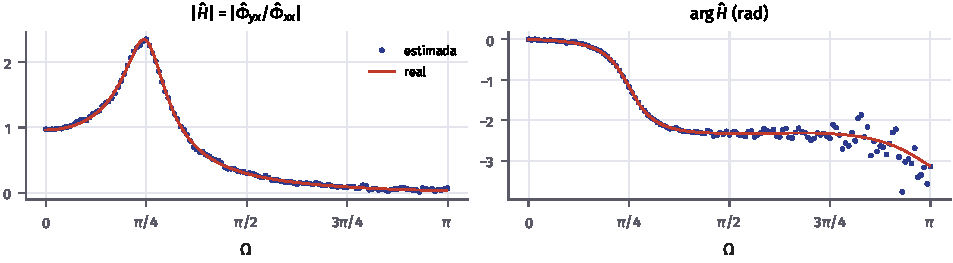
\includegraphics[width=\linewidth]{identificacion}
  \caption{Respuesta en frecuencia de $H(z)=(0{,}2+0{,}3z^{-1})/(1-1{,}2z^{-1}+0{,}72z^{-2})$ estimada con 20\,000 muestras de ruido blanco y ruido de medida de desviación típica 0,3.}\label{fig:identificacion}
\end{figure}

\begin{encodigo}
  Identificación con \texttt{tfestimate} (Matlab) y con \texttt{csd}/\texttt{welch} (Python). \texttt{scipy.signal.csd(x, y)} promedia $X^*Y$, que con nuestro convenio estima $\Phi_{yx}$.
  \codigo{identificacion}
\end{encodigo}

\subsection{Estimación de la densidad espectral}

\paragraph{Periodograma.} Con $N$ muestras de una realización, la estimación inmediata, sugerida por el teorema de Wiener-Khinchin, es el \emph{periodograma}
\[
  I_N(\e^{j\Omega})=\frac1N\abs{\sum_{n=0}^{N-1}x[n]\,\e^{-j\Omega n}}^2 ,
\]
que se calcula en las frecuencias $\Omega_k=2\pi k/N$ con la FFT. Se puede comprobar que es la DTFT del estimador sesgado de la autocorrelación. Es asintóticamente insesgado: su media tiende a $\Phi_{xx}$ cuando $N$ crece. Pero su varianza no disminuye con $N$, sino que es del orden de $\Phi_{xx}^2$: con más muestras se obtienen más frecuencias, cada una tan ruidosa como antes (\cref{fig:periodograma}). Además, al truncar la señal, su media es la convolución de $\Phi_{xx}$ con el espectro de la ventana rectangular, con las fugas del Tema~3.

\begin{figure}[ht]
  \centering
  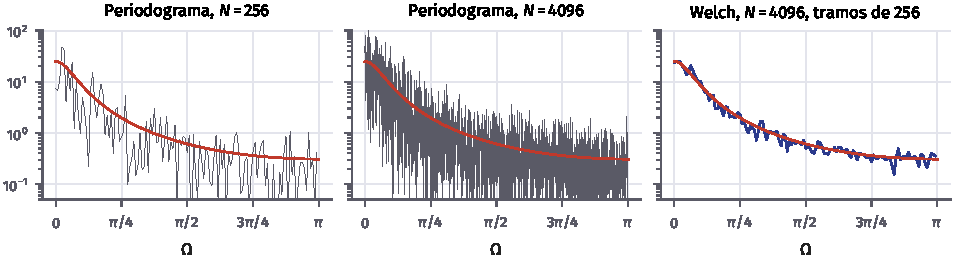
\includegraphics[width=\linewidth]{periodograma}
  \caption{Periodogramas de un AR(1) con $a=0{,}8$ y $N=256$ y 4096 muestras, y estimación de Welch. En rojo, la DEP teórica.}\label{fig:periodograma}
\end{figure}

\paragraph{Métodos de Bartlett y Welch.} Para reducir la varianza se promedia. El método de \emph{Bartlett} divide la señal en $K$ tramos de $L$ muestras, calcula el periodograma de cada uno y los promedia; si los tramos son aproximadamente independientes, la varianza baja en un factor $K$, a cambio de una resolución en frecuencia de $\approx2\pi/L$ en lugar de $2\pi/N$. El de \emph{Welch} enventana cada tramo (Hann, Hamming), para reducir las fugas, y los solapa, típicamente un 50\,\%, para aprovechar mejor los datos. Es el mismo compromiso entre resolución y estabilidad que el del espectrograma del Tema~5. Las densidades cruzadas se estiman igual promediando $X_m^*(\e^{j\Omega})Y_m(\e^{j\Omega})$ de cada tramo.

En Matlab: \texttt{periodogram}, \texttt{pwelch}, \texttt{cpsd}, \texttt{tfestimate} y \texttt{mscohere}; en Python, las funciones de mismo nombre de \texttt{scipy.signal}: \texttt{periodogram}, \texttt{welch}, \texttt{csd} y \texttt{coherence}. Por defecto devuelven la DEP \emph{unilateral} (el doble de $\Phi_{xx}$ entre 0 y $f_s/2$, para que la integral en ese intervalo dé la potencia) y por unidad de frecuencia: por hercio si se da $f_s$, y en Matlab por rad/muestra si no se da. Con la opción bilateral (\texttt{'twosided'}, \texttt{return\_onesided=False}) y $f_s=1$, el resultado es directamente $\Phi_{xx}(\e^{j2\pi f})$ con $f$ en ciclos por muestra. Además, \texttt{scipy.signal.welch} resta por defecto la media de cada tramo (\texttt{detrend='constant'}), que elimina la componente continua; con \texttt{detrend=False} se conserva. El solapamiento se indica en muestras en Matlab y como fracción en Octave; dejándolo vacío (\texttt{[]}) ambos usan el 50\,\%.

\begin{encodigo}
  DEP de un AR(1) con $a=0{,}8$ estimada con Welch y comparada con la teórica: $\Phi_{xx}(\e^{j0})=1/(1-a)^2=25$, $\Phi_{xx}(\e^{j\pi/2})=1/(1+a^2)=0{,}61$ y potencia $1/(1-a^2)=2{,}78$. El valor en $\Omega=0$, donde hay un pico estrecho, es el que peor se estima.
  \codigo{welch}
\end{encodigo}

\subsection{Aplicaciones}

\begin{itemize}
  \item \emph{Medida de ruido}: la DEP del ruido de un sistema y su relación señal a ruido en cada banda.
  \item \emph{Detección de tonos} débiles: al promediar, la varianza del fondo de ruido disminuye y un tono que estaba oculto en un periodograma aislado destaca.
  \item \emph{Identificación} de sistemas en funcionamiento, añadiendo una pequeña señal aleatoria a la entrada.
  \item \emph{Filtro de Wiener}: si una señal $s$ se observa con un ruido aditivo $v$ incorrelado, $x=s+v$, el filtro lineal que minimiza el error cuadrático medio de la estimación de $s$ es
  \[
    H(\e^{j\Omega})=\frac{\Phi_{ss}(\e^{j\Omega})}{\Phi_{ss}(\e^{j\Omega})+\Phi_{vv}(\e^{j\Omega})},
  \]
  que deja pasar las frecuencias en las que domina la señal y atenúa aquellas en las que domina el ruido. Es la idea de los reductores de ruido y de la restauración de imágenes del Tema~5.
\end{itemize}

\begin{flushright}\small\color{pdsgris}Ejercicios 15–18.\end{flushright}

% =====================================================================
\section*{Bibliografía}
\addcontentsline{toc}{section}{Bibliografía}

\begin{itemize}
  \item A.~V. Oppenheim y R.~W. Schafer, \emph{Tratamiento de señales en tiempo discreto}, 3.ª ed. Pearson, 2011. Apéndice A (señales aleatorias) y capítulo 10 (estimación espectral). De aquí procede el convenio de la correlación cruzada.
  \item J.~G. Proakis y D.~G. Manolakis, \emph{Tratamiento digital de señales}, 4.ª ed. Pearson Prentice Hall, 2007. Capítulos de señales aleatorias y de estimación del espectro de potencia.
  \item A.~Papoulis y S.~U. Pillai, \emph{Probability, Random Variables and Stochastic Processes}, 4.ª ed. McGraw-Hill, 2002. Referencia completa de probabilidad y procesos estocásticos.
  \item A.~Gelb (ed.), \emph{Applied Optimal Estimation}. MIT Press, 1974. Capítulo de repaso de probabilidad y procesos aleatorios, con la notación $\phi$ y $\Phi$ de las versiones anteriores de este tema.
  \item C.~M. Bishop, \emph{Pattern Recognition and Machine Learning}. Springer, 2006. Capítulos 2 (distribuciones) y 11 (métodos de muestreo: inversa, rechazo, Monte Carlo).
\end{itemize}

\end{document}
